%% LyX 2.5.1 created this file.  For more info, see https://www.lyx.org/.
%% Do not edit unless you really know what you are doing.
\documentclass[10pt,english]{beamer}
\usepackage{lmodern}
\usepackage[T1]{fontenc}
\usepackage[utf8]{inputenc}
\setcounter{tocdepth}{1}
\usepackage{colortbl}
\usepackage{babel}
\usepackage{amsbsy}
\usepackage{amstext}
\usepackage{amssymb}
\usepackage{graphicx}
\usepackage[authoryear]{natbib}
\ifx\hypersetup\undefined
  \AtBeginDocument{%
    \hypersetup{}
  }
\else
  \hypersetup{}
\fi

\makeatletter

%%%%%%%%%%%%%%%%%%%%%%%%%%%%%% LyX specific LaTeX commands.
%% Because html converters don't know tabularnewline
\providecommand{\tabularnewline}{\\}

%%%%%%%%%%%%%%%%%%%%%%%%%%%%%% Textclass specific LaTeX commands.
% this default might be overridden by plain title style
\newcommand\makebeamertitle{\frame{\maketitle}}%
% (ERT) argument for the TOC
\AtBeginDocument{%
  \let\origtableofcontents=\tableofcontents
  \def\tableofcontents{\@ifnextchar[{\origtableofcontents}{\gobbletableofcontents}}
  \def\gobbletableofcontents#1{\origtableofcontents}
}

%%%%%%%%%%%%%%%%%%%%%%%%%%%%%% User specified LaTeX commands.



\usepackage{tikz}
\usetikzlibrary{positioning}
\usetikzlibrary{overlay-beamer-styles}
\usepackage{appendixnumberbeamer}

\usepackage{graphicx}
\usepackage{subfig}

\usetheme[progressbar=frametitle,block=fill,subsectionpage=progressbar]{metropolis}

% margin
\setbeamersize{text margin right=1.5cm}

% colors
\colorlet{DarkRed}{red!70!black}
\setbeamercolor{normal text}{fg=black}
\setbeamercolor{alerted text}{fg=DarkRed}
\setbeamercolor{progress bar}{fg=DarkRed}
\setbeamercolor{button}{bg=DarkRed}

% width of seperators
\makeatletter
\setlength{\metropolis@titleseparator@linewidth}{1pt}
\setlength{\metropolis@progressonsectionpage@linewidth}{1pt}
\setlength{\metropolis@progressinheadfoot@linewidth}{1pt}
\makeatother

% new alert block
\newlength\origleftmargini
\setlength\origleftmargini\leftmargini
\setbeamertemplate{itemize/enumerate body begin}{\setlength{\leftmargini}{4mm}}
\let\oldalertblock\alertblock
\let\oldendalertblock\endalertblock
\def\alertblock{\begingroup \setbeamertemplate{itemize/enumerate body begin}{\setlength{\leftmargini}{\origleftmargini}} \oldalertblock}
\def\endalertblock{\oldendalertblock \endgroup}
\setbeamertemplate{mini frame}{}
\setbeamertemplate{mini frame in current section}{}
\setbeamertemplate{mini frame in current subsection}{}
\setbeamercolor{section in head/foot}{fg=normal text.bg, bg=structure.fg}
\setbeamercolor{subsection in head/foot}{fg=normal text.bg, bg=structure.fg}

% footer
\makeatletter
\setbeamertemplate{footline}{%
    \begin{beamercolorbox}[colsep=1.5pt]{upper separation line head}
    \end{beamercolorbox}
    \begin{beamercolorbox}{section in head/foot}
      \vskip1pt\insertsectionnavigationhorizontal{\paperwidth}{}{\hskip0pt plus1filll \insertframenumber{} / \inserttotalframenumber \hskip2pt}\vskip3pt%
    \end{beamercolorbox}%
    \begin{beamercolorbox}[colsep=1.5pt]{lower separation line head}
    \end{beamercolorbox}
}
\makeatother

% toc
\setbeamertemplate{section in toc}{\hspace*{1em}\inserttocsectionnumber.~\inserttocsection\par}
\setbeamertemplate{subsection in toc}{\hspace*{2em}\inserttocsectionnumber.\inserttocsubsectionnumber.~\inserttocsubsection\par}

% code
\usepackage{xcolor}
\usepackage{listings}

\definecolor{codegray}{rgb}{0.5,0.5,0.5}
\definecolor{background}{HTML}{F5F5F5}
\definecolor{keyword}{HTML}{4B69C6}
\definecolor{string}{HTML}{448C27}
\definecolor{comment}{HTML}{448C27}

\usepackage{inconsolata}
\lstdefinestyle{mystyle}{
    commentstyle=\color{comment},
    keywordstyle=\color{keyword},
    stringstyle=\color{string},
    basicstyle=\ttfamily,
    breakatwhitespace=false,
    breaklines=true,
    captionpos=b,
    keepspaces=true,
    numbersep=5pt,
    showspaces=false,
    showstringspaces=false,
    showtabs=false,
    tabsize=4,
	showlines=true
}

\lstset{style=mystyle}
% Added by lyx2lyx
\setlength{\parskip}{\smallskipamount}
\setlength{\parindent}{0pt}

\makeatother

\begin{document}
\title{Consumption-Saving\vspace{-2mm}}
\subtitle{Adv. Macro: Heterogeneous Agent Models}
\author{Raphaël Huleux}
\date{2026}

{
\setbeamertemplate{footline}{}
\begin{frame}
\maketitle
\end{frame}
}

\addtocounter{framenumber}{-1}

\section{Introduction}
\begin{frame}{\alt<2>{We open the household block}{A model is a set of blocks}}

\vspace{2mm}
\begin{center}
\begin{tikzpicture}[
block/.style={draw,thick,rounded corners,minimum width=3.1cm,minimum height=1cm,align=center},
lbl/.style={font=\scriptsize,alt=<2>{text=black!20}{}},
dim/.style={alt=<2>{draw=black!20,text=black!20}{}},
hl/.style={alt=<2>{draw=DarkRed,very thick,fill=DarkRed!10,text=DarkRed}{}}]

\node[block,dim] (gov) at (3.4,1.85) {Government};
\node[block,hl] (hh) at (0,0) {Households};
\node[block,dim] (firm) at (6.8,0) {Firms};
\node[block,dim] (mkt) at (3.4,-1.85) {Market clearing};

\draw[->,thick,dim] (hh.north east) -- node[lbl,above,sloped]{$N_{t}$, $A_{t}$} (firm.north west);
\draw[->,thick,dim] (firm.south west) -- node[lbl,below,sloped]{$r_{t}$, $w_{t}$} (hh.south east);
\draw[->,thick,dim] (gov.west) -- node[lbl,above,sloped]{$\tau_{t}$, transfers} (hh.north);
\draw[->,thick,dim] (gov.east) -- node[lbl,above,sloped]{$B_{t}$, $G_{t}$} (firm.north);
\draw[->,thick,dim] (hh.south) -- node[lbl,below,sloped]{$C_{t}$, $A_{t}$} (mkt.west);
\draw[->,thick,dim] (firm.south) -- node[lbl,below,sloped]{$Y_{t}$, $K_{t}$} (mkt.east);

\end{tikzpicture}
\end{center}

\vspace{1mm}
\begin{overlayarea}{\textwidth}{1.85cm}
\only<1|handout:0>{\textbf{Every block is a set of equations }mapping inputs into outputs.}
\only<2>{%
\textbf{This course focuses on the household block.}

\vspace{2mm}
\textbf{The question: }\emph{when does the distribution matter for aggregates?}%
}
\end{overlayarea}
\end{frame}
%
\begin{frame}{Goals for today}
\begin{itemize}
\item <+->\textbf{Review consumption-saving theory}
\begin{enumerate}
\item The permanent income hypothesis, and what it gets wrong
\item The buffer-stock model: risk and borrowing constraints
\end{enumerate}
\item <+->\textbf{Solve the household problem in partial equilibrium}
\begin{enumerate}
\item Basics of dynamic programming
\item Value function iteration (VFI)
\item The endogenous grid method (EGM)
\end{enumerate}
\item <+->\textbf{Simulate the distribution and aggregate}
\begin{enumerate}
\item Monte Carlo
\item The histogram method (Young, 2010)
\end{enumerate}
\item <+->\textbf{Note: }partial equilibrium for now, prices are \emph{fixed}.

They become equilibrium objects in the next lecture.
\end{itemize}
\end{frame}
%
\begin{frame}{Literature}
\begin{itemize}
\item <+->\textbf{Generations of models:}
\begin{enumerate}
\item \textbf{Permanent income hypothesis (PIH)} (Friedman, 1957)\\
or life-cycle model (Modigliani and Brumberg, 1954)
\item \textbf{Buffer-stock consumption model} \\
Deaton (1991, 1992); Carroll (1992, 1997, 2019)
\item \textbf{Multiple-asset buffer-stock consumption models} \\
e.g. Kaplan and Violante (2014); Harmenberg and Öberg (2021)
\end{enumerate}
\item <+->\textbf{Consumption-and-saving over the life-cycle dynamic }\\
e.g. Gourinchas and Parker (2002); Druedahl and Martinello (2022)
\item <+->\textbf{Empirical} \textbf{MPCs and income risk}\\
e.g. Fagereng et al. (2021);\textbf{ }Guvenen et al. (2021)
\end{itemize}
\vspace{5mm}\textbf{Book:} {\color{DarkRed}\href{https://global.oup.com/academic/product/the-economics-of-consumption-9780199383153?cc=dk&lang=en&}{The Economics of Consumption}},
Jappelli and Pistaferri (2017)
\end{frame}
%
\begin{frame}<beamer>
\frametitle{Plan}
\tableofcontents[]
\end{frame}

\section{PIH}
\begin{frame}{Keynes vs Friedman}
\begin{itemize}
\item <+->\textbf{Keynesian consumption function:} $C_{t}=a+bY_{t}$

Consumption responds to \emph{current} income. Multiplier is $\frac{1}{1-b}$. \\
But it lacks micro-foundations!
\item <+->\textbf{Permanent income hypothesis }(Friedman, 1957)\textbf{:}
Consumption responds to the \emph{present value }of income.\\
Current income matters only through it.
\item <+->But: PIH implies too low MPCs. We will see how to fix it
\end{itemize}
\end{frame}

\begin{frame}{Consumption-saving}

\vspace{-8mm}
\begin{align*}
v_{0} & =\max_{\{c_{t}\}^{T-1}_{t=0}}\sum^{T-1}_{t=0}\beta^{t}u(c_{t})\\
 & \text{s.t.}\\
a_{t} & =(1+r)a_{t-1}+wz_{t}-c_{t}\\
a_{T-1} & \geq0, \quad a_{-1}\  \text{given}
\end{align*}

\begin{itemize}
\item <+->\vspace{-3mm}\textbf{Variables:}

Consumption: $c_{t}$

Productivity: $z_{t}$

End-of-period savings: $a_{t}$ (\emph{no debt at death})
\item <+->\textbf{Parameters:}

Discount factor: $\beta$

Wage: $w$

Interest rate: $r$ (define $R\equiv1+r$ as interest factor)
\end{itemize}
\end{frame}

\begin{frame}{IBC}

\begin{itemize}
\item <+->\textbf{Only the terminal condition really constrains: }without
$a_{T-1}\geq0$ the household would just borrow more and more
\item <+->\textbf{Substitution }implies \emph{Intertemporal Budget Constraint}
(IBC)
\begin{align*}
a_{T-1} & = & Ra_{T-2}+wz_{T-1}-c_{T-1}\\
 & = & R(Ra_{T-3}+wz_{T-2}-c_{T-2})+wz_{T-1}-c_{T-1}\\
 & = & R^{T}a_{-1}+\sum^{T-1}_{t=0}R^{T-1-t}(wz_{t}-c_{t})
\end{align*}
\item <+->Use \textbf{terminal condition }$a_{T-1}=0$ (equality due to utility
max.)
\begin{align*}
R^{-(T-1)}a_{T-1}=0 & \Leftrightarrow & \sum^{T-1}_{t=0}R^{-t}c_{t}=s_{0}+h_{0}
\end{align*}
where $s_{0}\equiv Ra_{-1}$ (after-interest assets)\\
and $h_{0}\equiv\sum^{T-1}_{t=0}R^{-t}wz_{t}$ (human capital)
\end{itemize}
\end{frame}
%
\begin{frame}{FOC and Euler-equation}

\[
\mathcal{L}=\sum^{T-1}_{t=0}\beta^{t}u(c_{t})+\lambda\left[s_{0}+h_{0}-\sum^{T-1}_{t=0}R^{-t}c_{t}\right]
\]
\begin{itemize}
\item <+->\vspace{-3mm}\textbf{It is a }\textbf{\emph{static }}\textbf{problem:}
\begin{enumerate}
\item \textbf{Information: }$s_{0}$ and $h_{0}$ are known at $t=0$
\item \textbf{Target:} Discounted utility, $\sum^{T-1}_{t=0}\beta^{t}u(c_{t})$
\item \textbf{Behavior:} Choose $c_{0},c_{1},\dots,c_{T-1}$ \emph{simultaneously}
\item \textbf{Solution: }Sequence of consumption \emph{choices} $c^{\ast}_{0},c^{\ast}_{1},\dots,c^{\ast}_{T-1}$
\end{enumerate}

\item <+->\textbf{First order conditions}:
\[
\forall t:0=\beta^{t}u^{\prime}(c_{t})-\lambda R^{-t}\Leftrightarrow u^{\prime}(c_{t})=\lambda\left(\beta R\right)^{-t}
\]
\item <+->\textbf{Euler-equation} for $k\in\{1,2,\dots\}$:
\[
\frac{u^{\prime}(c_{t})}{u^{\prime}(c_{t+k})}=\frac{\lambda\left(\beta R\right)^{-t}}{\lambda\left(\beta R\right)^{-(t+k)}}=\left(\beta R\right)^{k}
\]

\end{itemize}
\end{frame}
%
\begin{frame}{Consumption choice}
\begin{itemize}
\item <+->\textbf{CRRA:} $u(c_{t})=\frac{c^{1-\sigma}_{t}}{1-\sigma}$ imply
Euler-equation
\[
\frac{c^{-\sigma}_{0}}{c^{-\sigma}_{t}}=\left(\beta R\right)^{t}\Leftrightarrow c_{t}=(\beta R)^{\frac{t}{\sigma}}c_{0}
\]

Constant consumption if:
\begin{enumerate}
\item $\beta R=1$
\item $\frac{1}{\sigma}\rightarrow0$ (zero intertemporal elasticity of
substitution)
\end{enumerate}
\item <+->Insert \textbf{Euler }into\textbf{ IBC} to get consumption choice
\begin{align*}
\sum^{T-1}_{t=0}\left((\beta R)^{1/\sigma}R^{-1}\right)^{t}c_{0} & = && (s_{0}+h_{0})\Leftrightarrow\\
c^{\ast}_{0} & =  \frac{1-(\beta R)^{1/\sigma}R^{-1}}{1-\left((\beta R)^{1/\sigma}R^{-1}\right)^{T}}&&(s_{0}+h_{0})
\end{align*}
\end{itemize}
\end{frame}
%
\begin{frame}{Infinite horizon: $T\rightarrow\infty$}
\begin{itemize}
\item <+->\textbf{Infinite horizon }for $(\beta R)^{1/\sigma}R^{-1}<1$:

Let $T\rightarrow\infty$ to get
\begin{align*}
c^{\ast}_{0} & =\left(1-\frac{(\beta R)^{1/\sigma}}{R}\right)(s_{0}+h_{0})
\end{align*}
Assuming $\beta R =1$, this becomes
$$
c_{0} = \frac{r}{1+r}(s_{0}+h_{0})
$$
$\Rightarrow$ Consumption is the annuity value of total wealth (perfect consumption smoothing!)
\end{itemize}
\end{frame}
%
\begin{frame}{Consumption smoothing}

\begin{center}
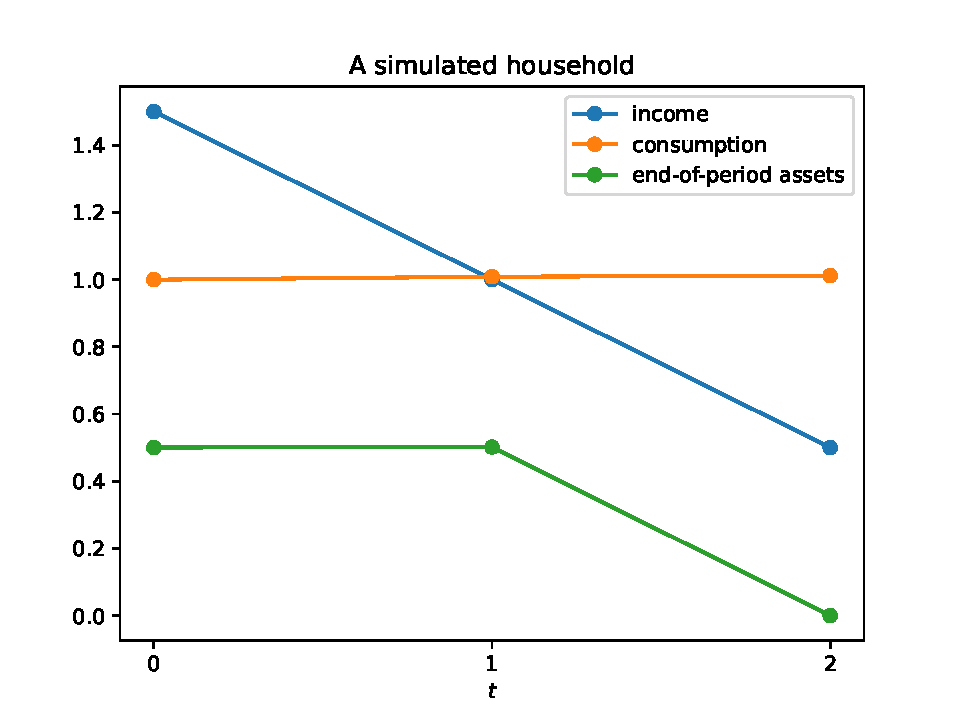
\includegraphics[width=0.72\textwidth]{figs/pih_simulation}
\end{center}

\textbf{Income falls by two thirds, consumption stays constant.}
The household saves while income is high and runs the savings down
when it is low. ($T=3$, $a_{-1}=0$, from \texttt{02\_vfi\_pih.ipynb})
\end{frame}
%
\begin{frame}{Propensities to consume ($\beta R=1$, $z_{t}=1$)}

Assume $\beta R=1$ and $z_{t}=1$, then
\[
c^{\ast}_{0}= ra_{-1}+w
\]

\textbf{MPC for different types of shocks} (exact derivatives):
\begin{enumerate}
\item <+->MPC of \emph{windfall} income: $\frac{\partial c_{0}}{\partial s_{0}}=\frac{r}{1+r}\approx r\%$
\item <+->MPC of \emph{future} income change: $\frac{\partial c_{0}}{\partial wz_{t}}=\frac{r}{1+r}\left(1+r\right)^{-t}$ $\to$ even smaller
\item <+->MPC of \emph{permanent} income change: $\frac{\partial c_{0}}{\partial w}=1$
\end{enumerate}

\end{frame}
%
\begin{frame}{Connection to the representative agent}
\begin{itemize}
\item <+->\textbf{The consumption function is }\emph{linear}\textbf{ in resources}
\[
c^{\ast}_{0}=\kappa\left(s_{0}+h_{0}\right),\qquad\kappa\equiv1-\frac{(\beta R)^{1/\sigma}}{R}
\]
with the \emph{same} $\kappa$ for every household
\item <+->\textbf{Exact aggregation: }sum over households $i$
\[
\sum_{i}c^{\ast}_{0,i}=\kappa\left(\sum_{i}s_{0,i}+\sum_{i}h_{0,i}\right)
\]
\item <+->\textbf{Implication: }aggregate consumption depends on \emph{aggregate }wealth and \emph{aggregate }income only. The distribution does not enter, and a representative agent gets the aggregates exactly right.
\item <+->\textbf{This is why the course exists: }\emph{heterogeneity matters for aggregates only once this linearity breaks.}
\end{itemize}
\end{frame}

\section{Dynamic programming}
\begin{frame}{Why we need a different method}
\begin{itemize}
\item <+->\textbf{What made the sequence approach work:}
\begin{enumerate}
\item Substitute the budget constraint forward into a single IBC
\item Impose one terminal condition
\item Solve the FOCs for the whole path at once
\end{enumerate}
\item <+->\textbf{Dynamic programming: }solve the problem \emph{recursively},
one period at a time
\item <+->Will be very useful when we introduce risk and occasionally binding
constraints
\end{itemize}
\end{frame}
%
\begin{frame}{Dynamic solution: Bellman's Principle of Optimality}
\begin{itemize}
\item <+->\textbf{Go back to a finite horizon }with $T$ periods, and solve it backwards from the terminal condition $v_{T}(\bullet)=0$
\item <+->\textbf{Principle: }\emph{whatever the initial state and initial decision, the remaining decisions must be optimal given the state that results from the first decision}
\item <+->\textbf{Value function, $v_{t}$: }defined \emph{recursively} from $v_{T}(\bullet)=0$
\begin{align*}
v_{t}(a_{t-1}) & =\max_{c_{t}}u(c_{t})+\beta v_{t+1}(a_{t})\\
 & \text{s.t. }a_{t}=(1+r)a_{t-1}+wz_{t}-c_{t}, \quad a_{T-1}\geq 0
\end{align*}
\item <+->\textbf{Policy function, $c^{\ast}_{t}(a_{t-1})$: }we are looking for a \textbf{function} of \textbf{state variables}, instead of a \textbf{sequence}
\item <+->\textbf{Euler-equation }(interior choice):
\begin{enumerate}
\item FOC: $c^{-\sigma}_{t}=\beta v_{t+1,a}(a_{t})$
\item Envelope: $v_{t,a}(a_{t-1})=(1+r)c^{-\sigma}_{t}$ (fix $c_{t}$)
\item Combine, shifting the envelope forward: $c^{-\sigma}_{t}=\beta(1+r)c^{-\sigma}_{t+1}$
\end{enumerate}
\end{itemize}

\end{frame}
%
\begin{frame}{Infinite horizon: value function iteration}

\vspace{-7mm}
\begin{align*}
v(a_{t-1}) & =\max_{c_{t}}u(c_{t})+\beta v(a_{t})\\
 & \text{s.t. }a_{t}=(1+r)a_{t-1}+wz_{t}-c_{t},\quad a_{t}\geq0
\end{align*}

\begin{itemize}
\item <+->\textbf{Contraction mapping result:} \emph{If $\beta$ is low enough (strong enough impatience) then the value and policy functions converge to $v(a_{t-1})$ and $c^{\ast}(a_{t-1})$ for large enough $T$}
\item <+->Problem becomes \textbf{stationary}
\item <+->\textbf{In practice: }for an infinite-horizon problem
\begin{enumerate}
\item Make an arbitrary initial guess (e.g. $v_{T}=0$)
\item Iterate the backward step until the value (and/or policy) function does not change anymore, relative to a chosen tolerance
\end{enumerate}
\end{itemize}
\end{frame}

\section{VFI}
\begin{frame}{Three numerical problems}
\begin{enumerate}
\item <+->\textbf{Discretize the state: }$a_{t-1}$ lives on a continuum, the
computer needs a \emph{grid}
\item <+->\textbf{Approximate off the grid: }$v_{t+1}$ is known only at grid
points, but $a_{t}=(1+r)a_{t-1}+wz_{t}-c_{t}$ lands between them
\item <+->\textbf{Maximize: }find $c^{\ast}_{t}$ at every grid point
\end{enumerate}
\vspace{3mm}
\textbf{Next lecture adds a fourth: }\emph{numerical integration},
once income is risky and the continuation value is an expectation.

\vspace{3mm}
\textbf{Notebooks: }\texttt{01\_tools.ipynb}, \texttt{02\_vfi\_pih.ipynb}
\end{frame}
%
\begin{frame}[fragile]{Grids}
\begin{itemize}
\item <+->\textbf{Discretization: }the state variable belongs to a discrete set
$\equiv$ a \emph{grid}\vspace{-2mm}
\begin{align*}
a_{t} & \in\mathcal{G}_{a}=\{a^{0},a^{1},\dots,a^{\#_{a}-1}\},\quad a^{0}=\underline{a}
\end{align*}
\item <+->\textbf{Not equally spaced: }the policy function bends most near the
borrowing constraint, so that is where the points should be
\item <+->\textbf{ConSav: }\lstinline{grids.nonlinspace}, \lstinline{grids.equilogspace}
\end{itemize}

\vspace{-1mm}

\includegraphics[width=0.85\textwidth]{figs/grids}
\end{frame}
%
\begin{frame}[fragile]{Linear interpolation}
\begin{itemize}
\item <+->\textbf{Linear interpolation }(function approximation):\vspace{1mm}
\begin{enumerate}
\item Assume $v_{t+1}$ is known on $\mathcal{G}_{a}$
\item Evaluate $v_{t+1}(a)$ for arbitrary $a$ by\vspace{-2mm}
\begin{align*}
\breve{v}_{t+1}(a) & =\text{baseline + slope}\times\text{distance}\\
 & =v_{t+1}(a^{\iota})+\omega(a-a^{\iota})\\
 & \text{where}\\
 & \omega\equiv\frac{v_{t+1}(a^{\iota+1})-v_{t+1}(a^{\iota})}{a^{\iota+1}-a^{\iota}}\\
 & \iota\equiv\text{largest }i_{a}\in\{0,1,\dots,\#_{a}-2\}\text{ such that }a^{i_{a}}\leq a
\end{align*}
\end{enumerate}
\item <+->\textbf{ConSav: }\lstinline{linear_interp.interp_1d}
\end{itemize}
\end{frame}
%
\begin{frame}{Linear interpolation}

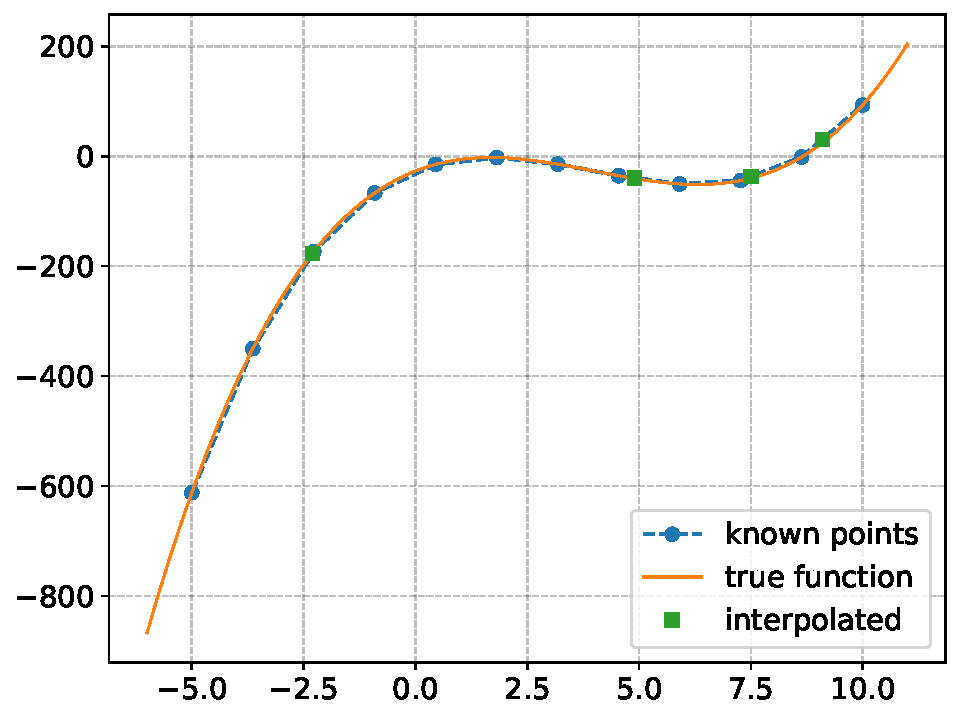
\includegraphics[width=0.95\textwidth]{figs/linear_interpolation}
\end{frame}
%
\begin{frame}[fragile]{Numerical optimization}
\begin{itemize}
\item <+->\textbf{Grid search: }try $\#_{c}$ values of $c_{t}$, keep the best
\begin{itemize}
\item Robust, but the accuracy is the spacing of the trial grid
\end{itemize}
\item <+->\textbf{Golden section search: }keep a bracket $[\underline{c},\overline{c}]$
known to contain the maximum, place two interior points, discard the
part that cannot contain it
\begin{itemize}
\item Bracket shrinks by $1/\varphi\approx0.618$ per iteration
\item Requires the objective to be \emph{unimodal}
\end{itemize}
\item <+->\textbf{Why derivative-free? }$\breve{v}_{t+1}$ is piecewise linear,
so its derivative is a step function
\item <+->\textbf{ConSav: }\lstinline{golden_section_search.optimizer}

Note: it \emph{minimizes}, so pass the negative of the value
\end{itemize}
\end{frame}
%
\begin{frame}[fragile]{Value function iteration (VFI)}
\begin{itemize}
\item <+->\textbf{Maximize the value-of-choice:}
\begin{align*}
v_{t}(a_{i_{a-}}) & =\max_{c_{t}}v_{t}(a_{i_{a-}}|c_{t})\\
 & \text{with }c_{t}\in\left[0,(1+r)a_{i_{a-}}+wz_{t}-\underline{a}\right]
\end{align*}
\vspace{-7mm}
\begin{align*}
v_{t}(a^{i_{a-}}|c_{t}) & =u(c_{t})+\beta\breve{v}_{t+1}(a_{t})\\
 & \text{with }a_{t}=(1+r)a^{i_{a-}}+wz_{t}-c_{t}
\end{align*}
\item <+->\textbf{Inner loop: }for each grid point in $\mathcal{G}_{a}$ find
$c^{\ast}_{t}(a_{t-1})$, and therefore $v_{t}(a_{t-1})$, with a \emph{numerical
optimizer}
\item <+->\textbf{Outer loop: }backwards from $t=T-1$ (note $v_{T}=0$, or known)
\end{itemize}
\end{frame}
%
\begin{frame}{It works}

\begin{tabular}{@{}c@{\hspace{2mm}}c@{}}
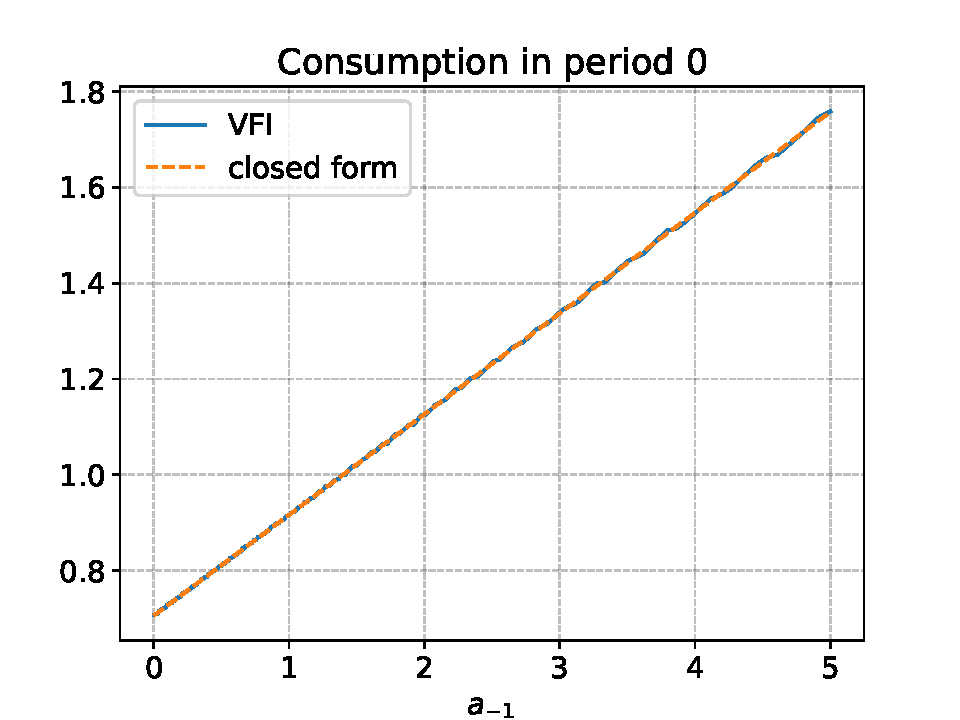
\includegraphics[width=0.48\textwidth]{figs/pih_vfi_vs_closed} & 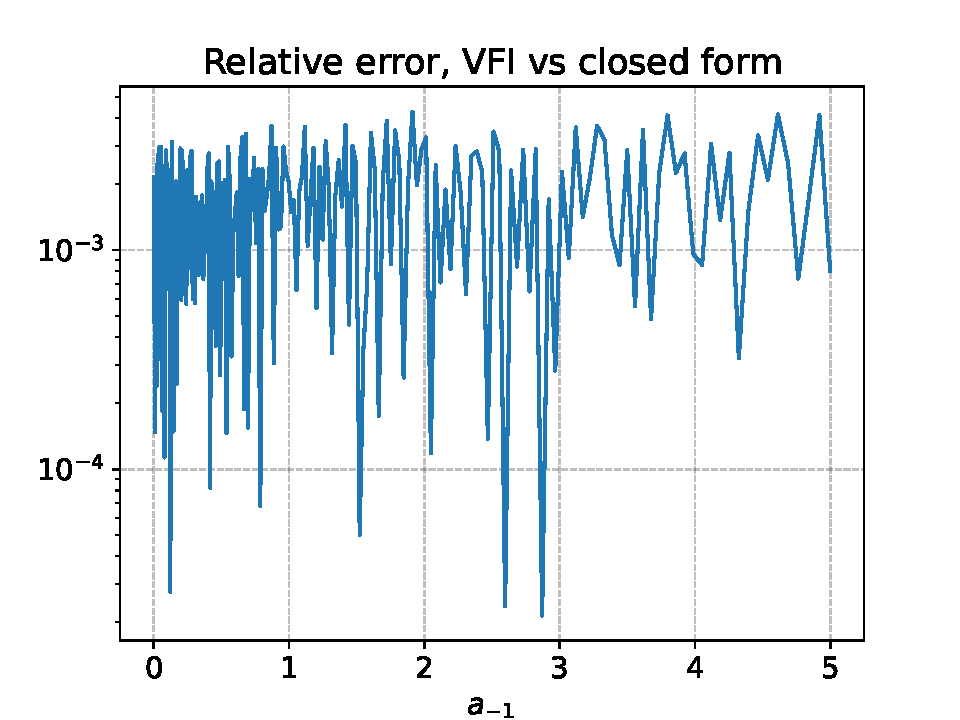
\includegraphics[width=0.48\textwidth]{figs/pih_vfi_error}\tabularnewline
\end{tabular}

\textbf{The only model in the course with a known answer.} $T=3$,
$\beta=0.99$, $r=0.02$, $\sigma=2$, falling income.

Maximum relative error: $3.6\times10^{-3}$ with $\#_{a}=200$.
\end{frame}
%
\begin{frame}{Accuracy and the number of grid points}

\begin{center}
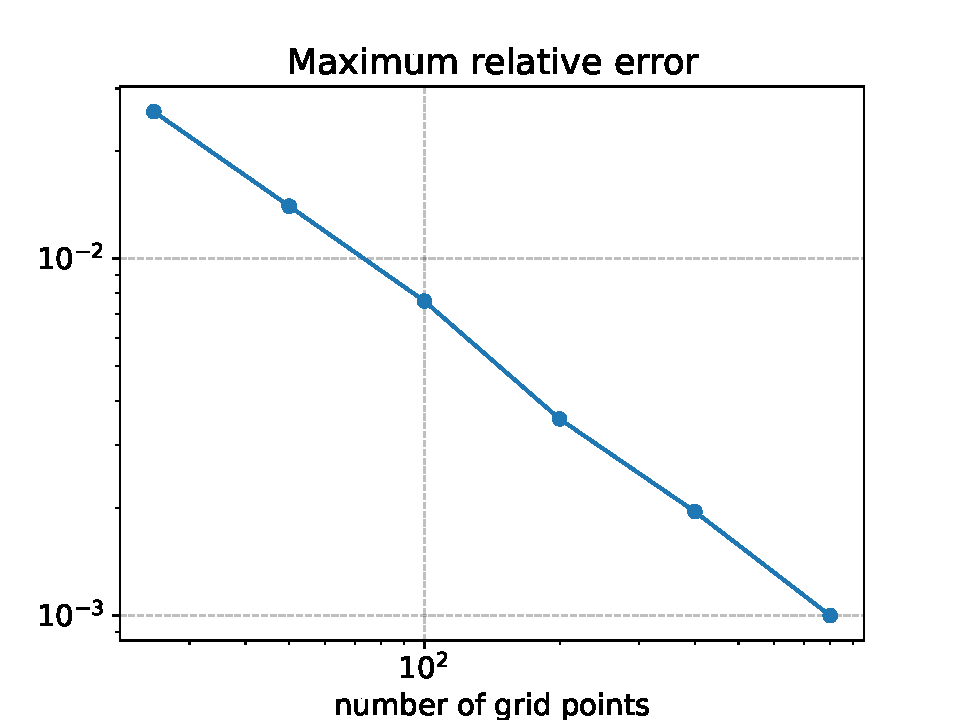
\includegraphics[width=0.62\textwidth]{figs/pih_vfi_convergence}
\end{center}

\begin{itemize}
\item <+->\textbf{Doubling the grid roughly halves the error}
\item <+->\textbf{The bottleneck is interpolating }$v_{t+1}$\textbf{, which is
strongly curved}
\item <+->$\Rightarrow$ \emph{three more digits would need a grid a thousand
times finer}
\end{itemize}
\end{frame}

\section{Buffer-stock}
\begin{frame}{MPCs in the data are high}

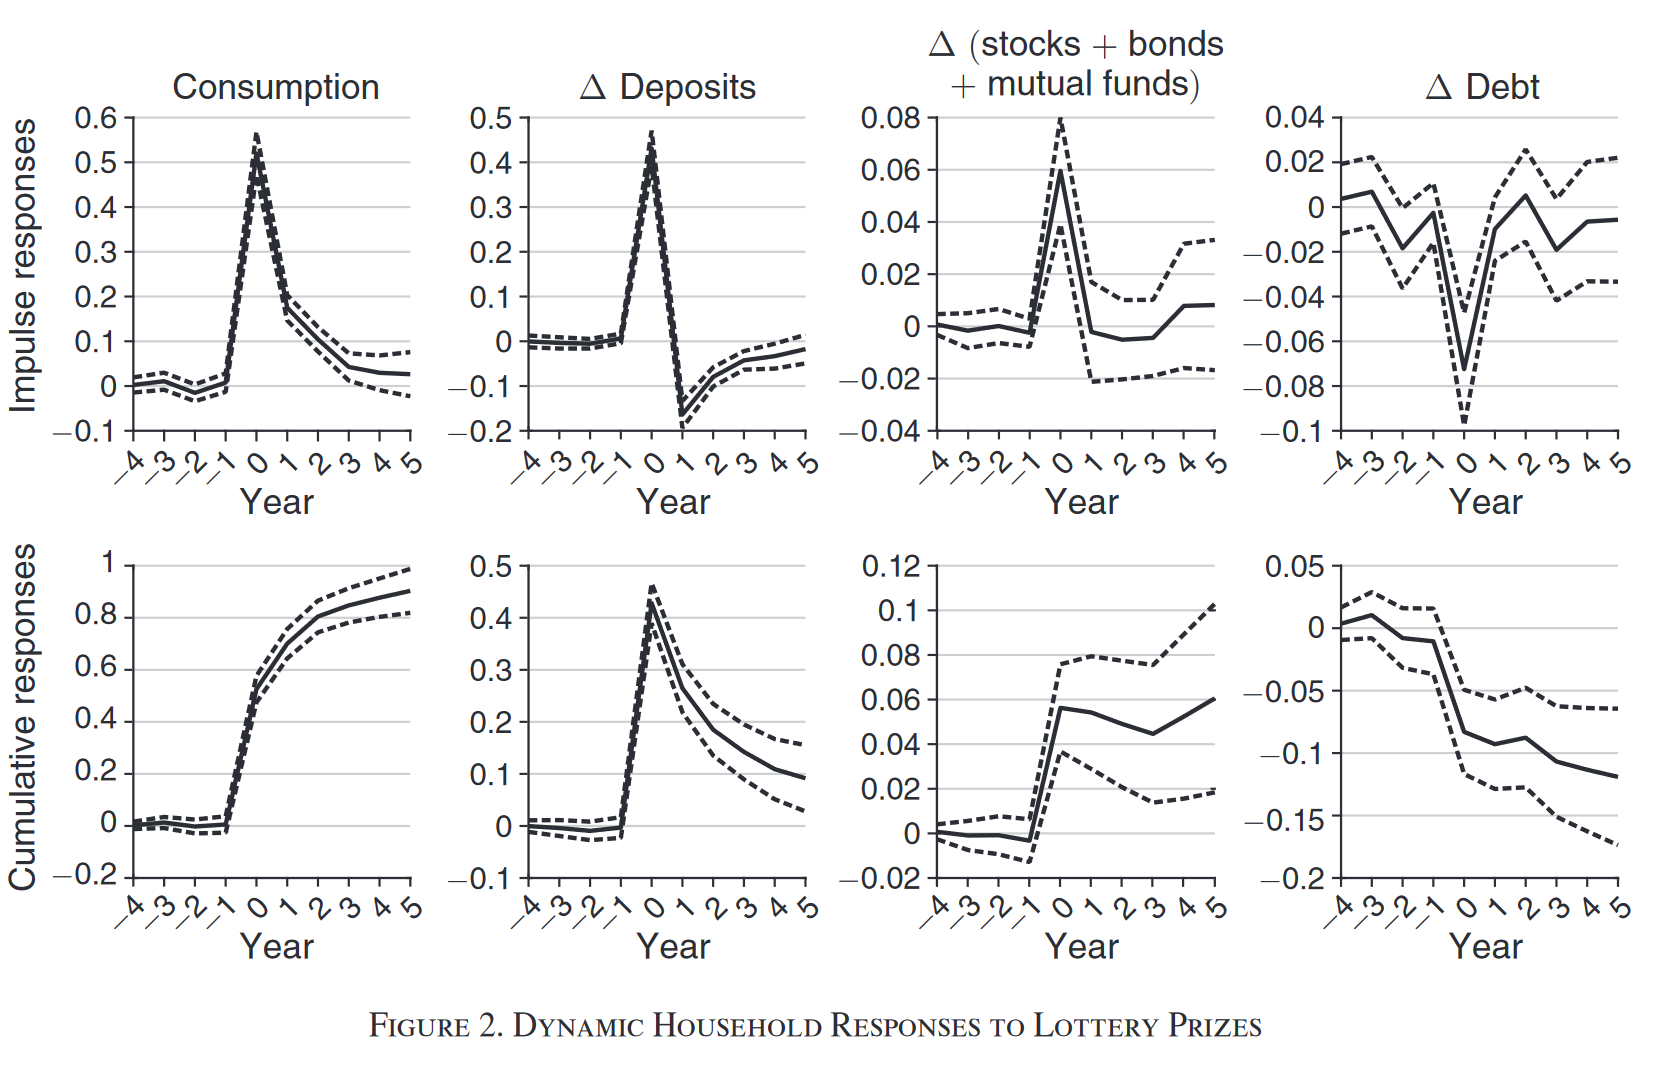
\includegraphics[width=1\textwidth]{figs/Fagereng_MPCs}

\textbf{Source:} Fagereng et al. (2021). \textbf{PIH says }$\frac{r}{1+r}\approx2\%$.
\end{frame}
%
\begin{frame}{What is missing from the model}
\begin{itemize}
\item <+->\textbf{Income risk }with a \emph{prudent }household

$\Rightarrow$ precautionary saving, relatively larger for the asset
poor
\item <+->\textbf{A borrowing constraint that can bind at any date}

$\Rightarrow$ MPC of one for the constrained, and a kink in the consumption
function
\item <+->\textbf{Both break the }\emph{linear}\textbf{ consumption function}

$\Rightarrow$ exact aggregation fails, and the distribution starts
to matter
\item <+->\textbf{The price: }no closed form.

\emph{That is why we spent the last lecture on numerical methods.}
\end{itemize}
\end{frame}
%
\begin{frame}{Uncertainty and a borrowing constraint}

\vspace{-8mm}
\begin{align*}
v_{0}(z_{0},a_{-1}) & =\max_{\{c_{t}\}^{\infty}_{t=0}}\mathbb{E}_{0}\left[\sum^{\infty}_{t=0}\beta^{t}u(c_{t})\right]\\
 & \text{s.t.}\\
a_{t} & =(1+r)a_{t-1}+wz_{t}-c_{t}\\
z_{t} & = \rho z_{t-1} + \sigma^z \epsilon_{t}\\
a_{t} & \geq-wb\\
\lim_{t\rightarrow\infty}(1+r)^{-t}a_{t} & \geq0\,\,\,\,\,[\text{No-Ponzi game}]
\end{align*}

\begin{itemize}
\item <+->\vspace{-3mm}\textbf{Stochastic income} from AR-1 process
\item <+->\textbf{Ad-hoc borrowing limit: }debt of at most $b\geq0$, in units
of the wage
\item <+->\textbf{\emph{A true dynamic problem:}}
\begin{enumerate}
\item \textbf{Information: }$z_{t}$ is revealed period-by-period
\item \textbf{Target:} \emph{Expected} discounted utility, $\mathbb{E}_{0}\left[\sum^{\infty}_{t=0}\beta^{t}u(c_{t})\right]$
\item \textbf{Behavior: }Choose $c_{t}$ \emph{sequentially} as information
is revealed
\item \textbf{Solution:} Consumption \emph{function}, $c^{\ast}(z_{t},a_{t-1})$
\end{enumerate}
\end{itemize}
\end{frame}
%
\begin{frame}{Recursive formulation}

\vspace{-7mm}
\begin{align*}
v(z_{t},a_{t-1}) & =\max_{c_{t}}u(c_{t})+\beta\mathbb{E}_{t}\left[v(z_{t+1},a_{t})\right]\\
 & \text{s.t. }a_{t}=(1+r)a_{t-1}+wz_{t}-c_{t}\geq\underline{a}
\end{align*}

\begin{enumerate}
\item <+->\vspace{-3mm}\textbf{State variables: }$z_{t}$ \emph{and} $a_{t-1}$
\item <+->\textbf{Control }(choice)\textbf{ variable:} $c_{t}$
\item <+->\textbf{Continuation value:} $\beta\mathbb{E}_{t}[v(z_{t+1},a_{t})]$
\item <+->\textbf{Parameters: }$r$, $w$, and stuff in $u(\bullet)$
\end{enumerate}
\vspace{2mm}
\textbf{Compare with last lecture: }the \emph{entire }cost of adding
risk is one extra state variable and one expectation operator.

\vspace{2mm}
\textbf{Note: }no time subscript on $v$. The problem is stationary,
so the policy function is the same in every period.
\end{frame}
%
\begin{frame}{IBC}
\begin{itemize}
\item <+->\textbf{Substitution }still implies (path-by-path, for any realization
of $z_{t}$):
\begin{align*}
R^{-(T-1)}a_{T-1}=0 & \Leftrightarrow & \sum^{T-1}_{t=0}R^{-t}c_{t}=s_{0}+h_{0}
\end{align*}
\item <+->\textbf{What if $T\rightarrow\infty$? }We must have $\lim_{T\rightarrow\infty}R^{-(T-1)}a_{T-1}=0$
\begin{enumerate}
\item $\lim_{T\rightarrow\infty}R^{-(T-1)}a_{T-1}>0$: Consumption can be
increased
\item $\lim_{T\rightarrow\infty}R^{-(T-1)}a_{T-1}<0$: Violates No-Ponzi
game condition
\end{enumerate}
\item <+->For $T\rightarrow\infty$ we have the\textbf{ IBC}:
\[
\sum^{\infty}_{t=0}R^{-t}c_{t}=Ra_{-1}+\sum^{\infty}_{t=0}R^{-t}wz_{t}
\]
\end{itemize}
\end{frame}
%
\begin{frame}{Natural borrowing limit}
\begin{itemize}
\item <+->Denote \textbf{minimum possible productivity }by\textbf{ $\underline{z}$}
\item <+->\textbf{Consumption must be non-negative} $\Rightarrow$\\
\emph{interest payments must be less than minimum income}
\[
c_{t}\geq0\Rightarrow r(-a_{t})\leq w\underline{z}\Leftrightarrow a_{t}\geq-\frac{w\underline{z}}{r}
\]
If debt was larger it would in the worst case ($\forall z_{t}=\underline{z}$)
grow without bound even with zero consumption ($\forall c_{t}=0$)
\begin{align*}
a_{0} & =-\frac{w\underline{z}}{r}-\Delta\\
a_{1} & =(1+r)a_{0}+w\underline{z}=-\frac{w\underline{z}}{r}-(1+r)\Delta\\
a_{2} & =(1+r)a_{1}+w\underline{z}=-\frac{w\underline{z}}{r}-(1+r)^{2}\Delta\\
\vdots
\end{align*}
\item <+->\vspace{-2mm}\textbf{Natural borrowing constraint: $a_{t}\geq\underline{a}=-w\min\left\{ b,\frac{\underline{z}}{r}\right\} $}
\end{itemize}
\end{frame}
%
\begin{frame}{Euler-equation with an occasionally binding constraint}
\begin{itemize}
\item <+->\textbf{Attach a multiplier }$\mu_{t}\geq0$\textbf{ to }$a_{t}\geq\underline{a}$
\begin{align*}
\text{FOC:} & \,\,\,c^{-\sigma}_{t}=\beta\mathbb{E}_{t}\left[v_{a}(z_{t+1},a_{t})\right]+\mu_{t}\\
\text{Slackness:} & \,\,\,\mu_{t}\left(a_{t}-\underline{a}\right)=0\\
\text{Envelope:} & \,\,\,v_{a}(z_{t},a_{t-1})=(1+r)c^{-\sigma}_{t}
\end{align*}
\item <+->\textbf{Two cases:}
\begin{enumerate}
\item \textbf{Unconstrained }($a_{t}>\underline{a}$, so $\mu_{t}=0$):
\[
c^{-\sigma}_{t}=\beta R\,\mathbb{E}_{t}\left[c^{-\sigma}_{t+1}\right]
\]
\item \textbf{Constrained }($a_{t}=\underline{a}$, so $\mu_{t}>0$):
\[
c^{-\sigma}_{t}>\beta R\,\mathbb{E}_{t}\left[c^{-\sigma}_{t+1}\right]\,\,\,\text{and}\,\,\,c_{t}=(1+r)a_{t-1}+wz_{t}-\underline{a}
\]
\end{enumerate}
\item <+->\textbf{Why an inequality? }\emph{Lowering $c_{t}$ is always feasible,
raising it is not.} The household would like to borrow and cannot.
\end{itemize}
\end{frame}
%
\begin{frame}{Prudence and precautionary saving}
\begin{itemize}
\item <+->\textbf{Prudence: }$u^{\prime\prime\prime}(c)>0$, i.e. marginal utility
is \emph{convex}

CRRA has $u^{\prime\prime\prime}(c)=\sigma(\sigma+1)c^{-\sigma-2}>0$
\item <+->\textbf{Jensen on the Euler-equation }(take $\beta R=1$, unconstrained):
\[
u^{\prime}(c_{t})=\mathbb{E}_{t}\left[u^{\prime}(c_{t+1})\right]>u^{\prime}\left(\mathbb{E}_{t}\left[c_{t+1}\right]\right)\Leftrightarrow\mathbb{E}_{t}\left[c_{t+1}\right]>c_{t}
\]
\item <+->\textbf{Interpretation: }the household \emph{tilts consumption into
the future} to build a buffer. Risk lowers consumption today even
with no constraint.
\item <+->\textbf{Two distinct channels, same direction:}
\begin{enumerate}
\item \textbf{Risk }$\times$\textbf{ prudence: }precautionary saving
\item \textbf{Borrowing constraint: }cannot smooth downwards
\end{enumerate}
\end{itemize}
\end{frame}
%
\begin{frame}{Special case I: Quadratic utility}
\begin{itemize}
\item <+->\textbf{Quadratic utility:} $u(c_{t})=-\frac{1}{2}(\overline{c}-c)^{2}$
with $\beta R=1$ and >>large<< $\overline{c}$
\item <+->\textbf{Euler-equation: }\emph{Consumption = expected future consumption}
\begin{align*}
(\overline{c}-c_{t}) & =\mathbb{E}_{t}\left[(\overline{c}-c_{t+k})\right]\Leftrightarrow c_{t}=\mathbb{E}_{t}\left[c_{t+k}\right]
\end{align*}
\item <+->Use \textbf{IBC }in expectation\textbf{ }to get \textbf{consumption
function:}
\begin{align*}
\sum_{s=0}^{\infty}R^{-s}\mathbb{E}_{0}\left[c_{s}\right] &=Ra_{-1}+\sum_{s=0}^{\infty}R^{-s}w\mathbb{E}_{0}\left[z_{s}\right]\Rightarrow\\
c^{\ast}(z_{0},a_{-1})=c_{0} &=ra_{-1}+\frac{r}{R}\sum_{s=0}^{\infty}R^{-s}w\mathbb{E}_{0}\left[z_{s}\right]
\end{align*}
where we formally disregard the borrowing constraint
\item <+->\textbf{Certainty equivalence:} \emph{Only expected income matters}.
No prudence: $u^{\prime\prime\prime}=0$.
\end{itemize}
\end{frame}
%
\begin{frame}{Special case II: CARA utility}
\begin{itemize}
\item <+->\textbf{CARA utility:} $u(c_{t})=-\frac{1}{\alpha}e^{-\alpha c}$
\item <+->\textbf{Productivity is absolute random walk:}
\begin{align*}
z_{t} & =z_{t-1}+\psi_{t}\\
\psi_{t} & \sim\mathcal{N}(0,\sigma^{2}_{\psi})
\end{align*}
\item <+->\textbf{Consumption function }({\color{DarkRed}\href{https://www.econ2.jhu.edu/people/ccarroll/public/LectureNotes/Consumption/CARAModelWithYRisk/}{see proof}})\textbf{:}
\[
c^{*}(a_{t-1},z_{t})=ra_{t-1}+wz_{t}-\frac{\frac{1}{\alpha}\log\left(\beta R\right)+\frac{\alpha w^{2}\sigma^{2}_{\psi}}{2}}{r}
\]
where we formally disregard the borrowing constraint
\item <+->\textbf{Precautionary saving: }$\sigma^{2}_{\psi}\uparrow$ implies
$c^{*}_{t}\downarrow$ for given $z_{t}$ and $a_{t-1}$

$\Rightarrow$ \emph{accumulation of buffer-stock}
\item <+->\textbf{But: }the MPC is still \emph{constant}. Heterogeneous MPCs
need CRRA $+$ a constraint, and then a computer.
\end{itemize}
\end{frame}
%
\begin{frame}{Buffer-stock behavior}
\begin{itemize}
\item <+->\textbf{Two forces on assets:}
\begin{enumerate}
\item \textbf{Impatience }($\beta R<1$): pushes assets \emph{down}
\item \textbf{Prudence }$\times$\textbf{ risk}: pushes assets \emph{up}
\end{enumerate}
\item <+->\textbf{Buffer-stock target: }they balance at a level $a^{\ast}$ where
$\mathbb{E}_{t}\left[a_{t}\right]=a_{t-1}$
\begin{itemize}
\item Below $a^{\ast}$: the household builds its buffer
\item Above $a^{\ast}$: the household runs it down
\end{itemize}
\item <+->\textbf{Carroll's impatience condition: }a target exists if the household
is impatient enough to decumulate without risk, but prudent enough
to save against it
\item <+->\textbf{What to look for in the numerical solution:}
\begin{enumerate}
\item Consumption \emph{concave }in assets
\item MPC \emph{decreasing }in assets, and one at the constraint
\item Net savings crossing zero
\end{enumerate}
\end{itemize}
\end{frame}
%
\begin{frame}{Recursive formulation with $\underline{v}$}
\begin{itemize}
\item <+->\textbf{Beginning-of-period value function}
\[
\underline{v}\left(z_{t},a_{t}\right)=\mathbb{E}\left[v(z_{t+1},a_{t})\,|\,z_{t}\right]
\]
\item <+->\textbf{Value function}:
\begin{align*}
v(z_{t},a_{t-1}) & =\max_{c_{t}}u(c_{t})+\beta\underline{v}\left(z_{t},a_{t}\right)\\
 & \text{s.t. }a_{t}=(1+r)a_{t-1}+wz_{t}-c_{t}\geq\underline{a}
\end{align*}
\item <+->\textbf{Why do this? }\emph{Only one interpolation per guess of $c_{t}$}

Integrating \emph{inside} the maximization would cost $\#_{z}$ interpolations
per guess.
\item <+->\textbf{This is the convention }\lstinline{GEModelTools}\textbf{ uses
from the next lecture on}
\end{itemize}
\end{frame}
%
\begin{frame}{What risk costs us numerically}
\begin{itemize}
\item <+->\textbf{The state is now two-dimensional: }$\mathcal{G}_{z}\times\mathcal{G}_{a}$
(tensor product)
\item <+->\textbf{The continuation value is an expectation.} Two new jobs:
\begin{enumerate}
\item Turn the AR(1) into a \emph{finite Markov chain}
\item Turn $\mathbb{E}_{t}$ into a \emph{sum}\vspace{-1mm}
\[
\underline{v}(z^{i_{z}},a_{t})=\sum^{\#_{z}-1}_{i_{z+}=0}\pi_{i_{z},i_{z+}}v(z^{i_{z+}},a_{t})
\]
which is one matrix multiplication
\end{enumerate}
\item <+->\textbf{Everything else from last lecture carries over unchanged: }grids,
interpolation, the optimizer
\end{itemize}
\end{frame}
%
\begin{frame}[fragile]{Discretizing an AR(1)}
\begin{itemize}
\item <+->\textbf{Income process:}
\[
\log z_{t}=\rho_{z}\log z_{t-1}+\psi_{t},\,\,\,\psi_{t}\sim\mathcal{N}(0,\sigma^{2}_{\psi}),\,\,\,\mathbb{E}\left[z_{t}\right]=1
\]
\item <+->\textbf{Tauchen (1986): }evenly spaced grid spanning the unconditional
distribution, match the transition probabilities by integrating the
normal density
\item <+->\textbf{Rouwenhorst (1995): }build the transition matrix by recursion,
matching the persistence and the unconditional variance \emph{exactly}
\begin{itemize}
\item Preferred at high $\rho_{z}$, where Tauchen needs many nodes
\end{itemize}
\item <+->\textbf{ConSav: }\lstinline{markov.log_rouwenhorst}, \lstinline{markov.tauchen}
\end{itemize}

\vspace{-4mm}
\begin{center}
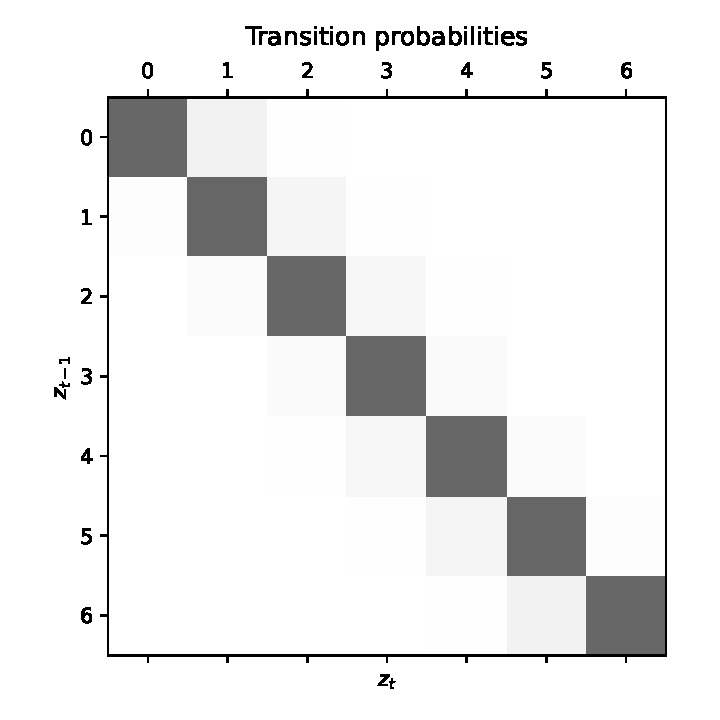
\includegraphics[width=0.33\textwidth]{figs/bs_z_trans}
\end{center}
\end{frame}
%
\begin{frame}[fragile]{VFI with risk}
\begin{itemize}
\item <+->\textbf{Maximize the value-of-choice:}
\begin{align*}
v(z^{i_{z}},a^{i_{a-}}) & =\max_{c_{t}}v(z^{i_{z}},a^{i_{a-}}|c_{t})\\
 & \text{with }c_{t}\in\left[0,(1+r)a^{i_{a-}}+wz^{i_{z}}-\underline{a}\right]
\end{align*}
\vspace{-7mm}
\begin{align*}
v(z^{i_{z}},a^{i_{a-}}|c_{t}) & =u(c_{t})+\beta\breve{\underline{v}}(z^{i_{z}},a_{t})\\
 & \text{with }a_{t}=(1+r)a^{i_{a-}}+wz^{i_{z}}-c_{t}
\end{align*}
\item <+->\textbf{Expectation step: }$\underline{v}=\Pi_{z}v$, before the maximization
\item <+->\textbf{Inner loop: }over $\mathcal{G}_{z}\times\mathcal{G}_{a}$ instead
of $\mathcal{G}_{a}$
\item <+->\textbf{Outer loop: }iterate until $v$ stops moving, instead of backwards
from $T$
\item <+->\textbf{Notebook: }\texttt{03\_vfi\_bufferstock.ipynb}
\end{itemize}
\end{frame}
%
\begin{frame}{Consumption function}

\begin{center}
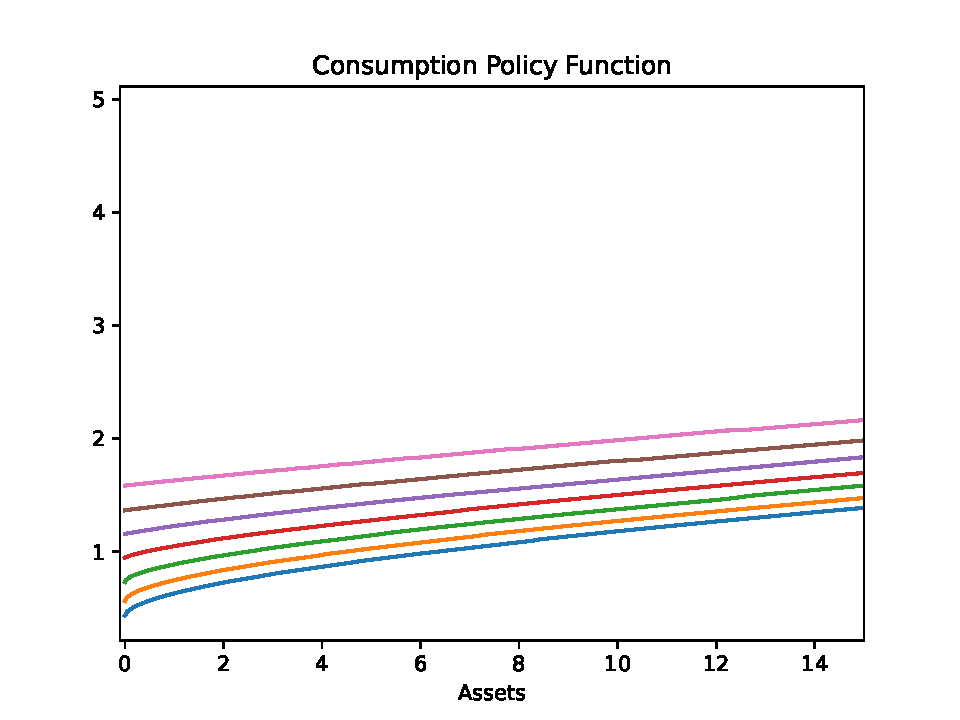
\includegraphics[width=0.72\textwidth]{figs/bs_c_func}
\end{center}

\textbf{Concave }in assets, and \textbf{kinked }where the borrowing
constraint starts to bind. One line per productivity state.
\end{frame}
%
\begin{frame}{Net savings and the buffer-stock target}

\begin{center}
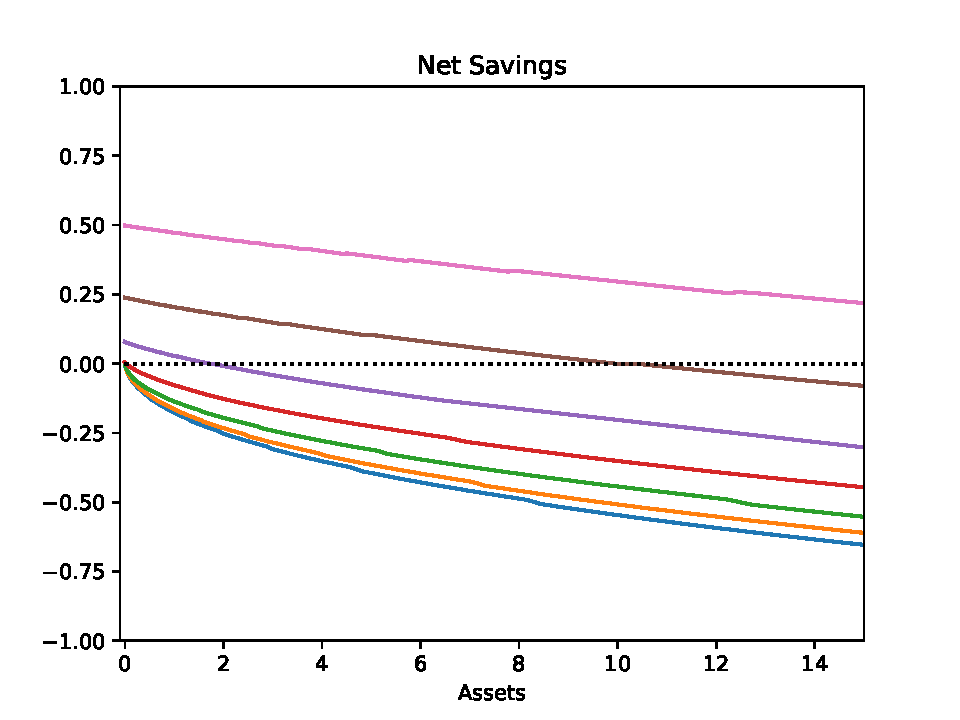
\includegraphics[width=0.72\textwidth]{figs/bs_a_func}
\end{center}

\textbf{Decreasing in wealth and crossing zero: }the crossing point
is the target. It exists despite $\beta R<1$.
\end{frame}
%
\begin{frame}{One household, simulated}

\begin{center}
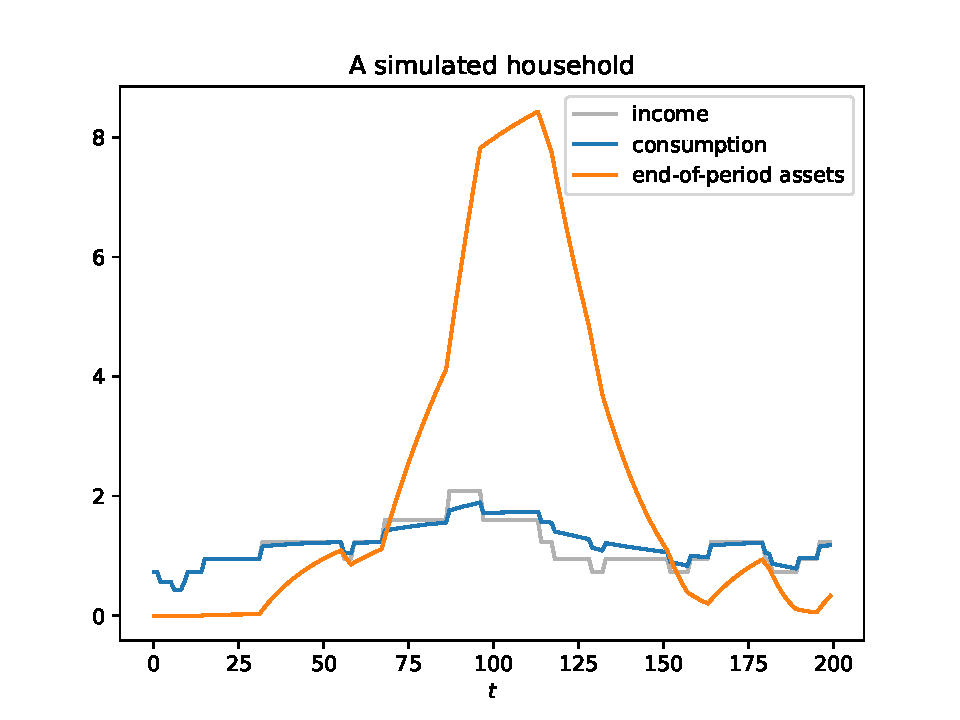
\includegraphics[width=0.72\textwidth]{figs/bs_simulation}
\end{center}

\textbf{Consumption is smoother than income, but not flat.}
The buffer is built in good times and run down in bad ones; when it
runs out, consumption tracks income one for one. (from \texttt{03\_vfi\_bufferstock.ipynb})
\end{frame}
%
\begin{frame}{MPC}

\begin{center}
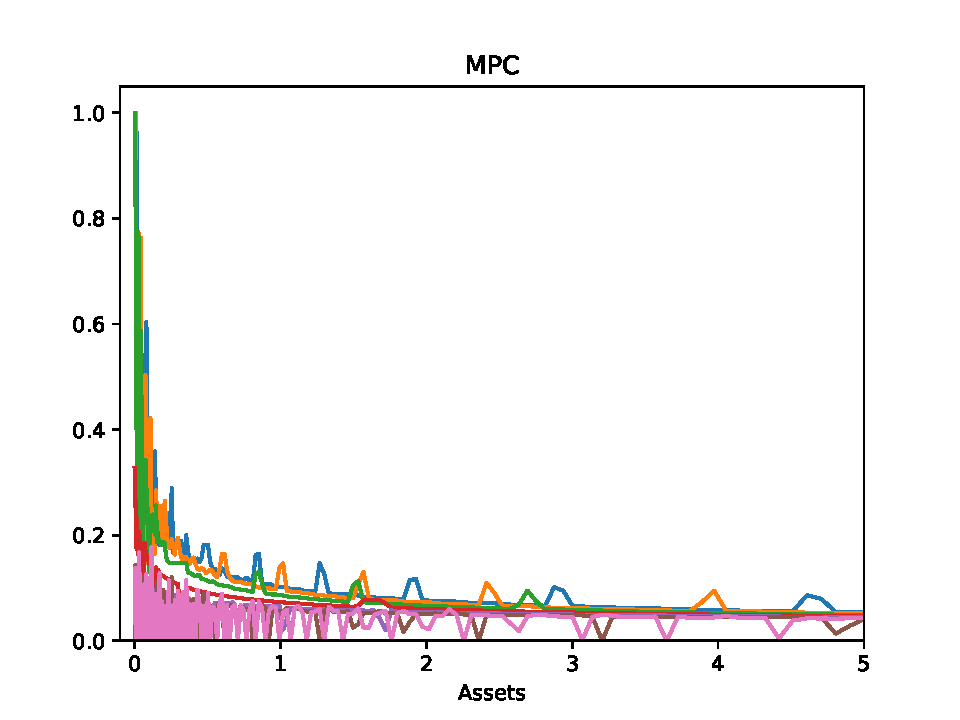
\includegraphics[width=0.72\textwidth]{figs/bs_MPC}
\end{center}

\textbf{One at the constraint, falling steeply with assets. }Under
the PIH it was $\frac{r}{1+r}$ for everybody.
\end{frame}
%
\begin{frame}{How much of this is risk?}

\begin{center}
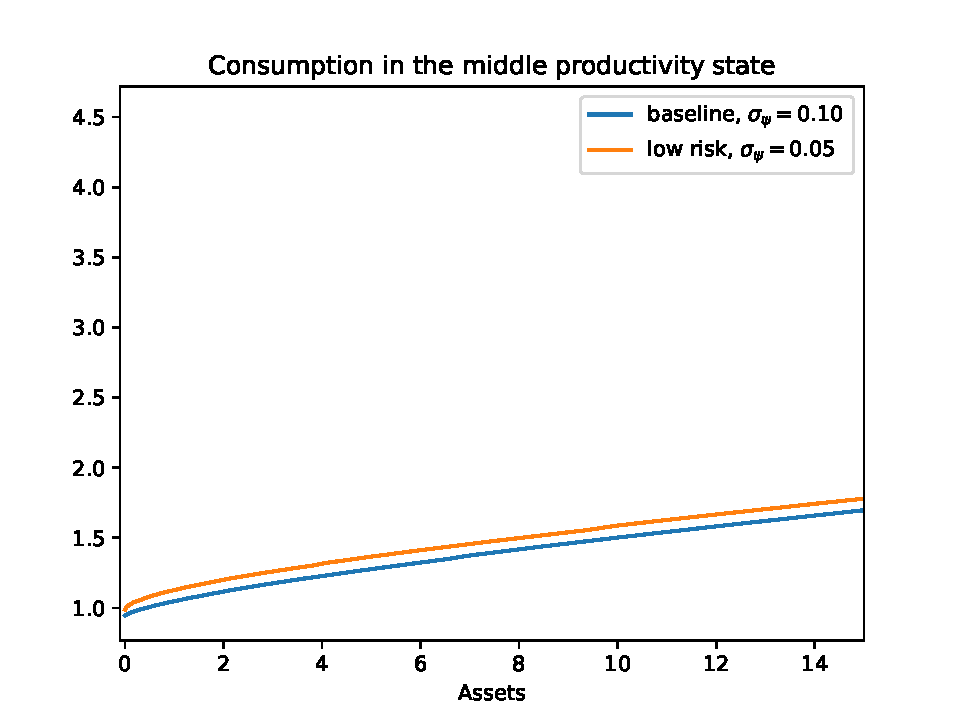
\includegraphics[width=0.72\textwidth]{figs/bs_c_func_risk}
\end{center}

\textbf{Halve }$\sigma_{\psi}$\textbf{ and consumption rises everywhere.}
The gap is largest for the asset poor: everybody faces the same risk,
but not everybody has a buffer against it.
\end{frame}
%
\begin{frame}{Economic insights}
\begin{itemize}
\item <+->\textbf{Consumption lower than under PIH and concave in assets}

\textbf{Intuition:} \emph{Precautionary saving motive is relatively
larger for asset poor households because income risk is the same for
everybody}

\textbf{Implications:}
\begin{enumerate}
\item Windfall gives safety and increases average consumption \\
$\Rightarrow$ MPC decreasing in assets
\item Attraction towards a buffer-stock target $a_{t}=a_{t-1}$ despite
$\beta R<1$
\item Larger effective discounting of future income

(extreme: no effect of future income changes if constrained before)
\end{enumerate}
\end{itemize}
\end{frame}
%
\begin{frame}{Taking stock}
\begin{itemize}
\item <+->\textbf{Value Function Iteration (VFI)}
\begin{enumerate}
\item Solves all consumption-saving models
\item Accurate with dense enough grids
\item Relatively simple code and easy to run in parallel
\item Finding optimal choices is the computational bottleneck\\
(especially with multi-starts in non-convex models)
\item Interpolating a strongly curved $v$ limits the accuracy
\end{enumerate}
\end{itemize}
\end{frame}

\section{EGM}
\begin{frame}{We can do better}
\begin{itemize}
\item <+->\textbf{Replace numerical optimization with root-finding}
\item <+->\textbf{Time iteration:} For each $a_{t-1}$ and $z_{t}$ find $c_{t}$
to solve the Euler-equation
\[
c^{-\sigma}_{t}=\beta(1+r)\mathbb{E}_{t}[c^{-\sigma}_{t+1}]
\]

Note: \emph{Necessary and sufficient} (for interior choices, else
$a_{t}=\underline{a}$)
\item <+->\textbf{EGM:} No need for any numerical optimization \emph{or} root-finding
\end{itemize}
\end{frame}
%
\begin{frame}{Endogenous grid-point method (EGM)}
\begin{enumerate}
\item <+->Calculate\textbf{ post-decision marginal value of cash:}\vspace{-1mm}
\[
q(z^{i_{z}},a^{i_{a}})=\sum^{\#_{z}-1}_{i_{z+}=0}\pi_{i_{z},i_{z+}}c^{\ast}_{+}(z^{i_{z+}},a^{i_{a}})^{-\sigma}
\]
\item <+->\vspace{-2mm}\textbf{Invert Euler-equation:}\vspace{-1mm}
\[
c(z^{i_{z}},a^{i_{a}})=(\beta(1+r)q(z^{i_{z}},a^{i_{a}}))^{-\frac{1}{\sigma}}
\]
\item <+->\vspace{-1mm}\textbf{Endogenous cash-on-hand:}\vspace{-1mm}
\[
m(z^{i_{z}},a^{i_{a}})=a^{i_{a}}+c(z^{i_{z}},a^{i_{a}})
\]
\item <+->\vspace{-1mm}\textbf{Consumption function:} Calculate $m=(1+r)a^{i_{a-}}+wz^{i_{z}}$\vspace{1mm}
\begin{enumerate}
\item Binding constraint: If $m\leq m(z^{i_{z}},a^{0})$ then\vspace{-1mm}
\[
c^{\ast}(z^{i_{z}},a^{i_{a-}})=m-\underline{a}
\]
\item \vspace{-3mm}Interior choice: Else\vspace{-1mm}
\[
c^{\ast}(z^{i_{z}},a^{i_{a-}})=\text{interpolate }m(z^{i_{z}},\bullet)\rightarrow c(z^{i_{z}},\bullet)\text{ at }m
\]
\end{enumerate}
\end{enumerate}
\end{frame}
%
\begin{frame}{Why it works}
\begin{itemize}
\item <+->\textbf{Fix }$a_{t}$\textbf{ instead of }$m_{t}$\textbf{.} Then the
expectation is taken \emph{before} the choice, and the FOC inverts
in closed form.
\begin{enumerate}
\item No optimizer, no root-finder
\item One interpolation per grid point
\end{enumerate}
\item <+->\textbf{It also interpolates the }\emph{policy}\textbf{ function rather
than the }\emph{value}\textbf{ function}

$\Rightarrow$ much more accurate, because $c^{\ast}$ is close to
linear while $v$ is strongly curved
\item <+->\textbf{Where it breaks: }non-concave problems and discrete choices,
where the FOC is not sufficient
\begin{itemize}
\item Fix: the \emph{upper envelope} method, see lecture 13
\end{itemize}
\item <+->\textbf{Notebook: }\texttt{04\_egm.ipynb}
\end{itemize}
\end{frame}
%
\begin{frame}{VFI vs EGM}

\begin{tabular}{@{}c@{\hspace{2mm}}c@{}}
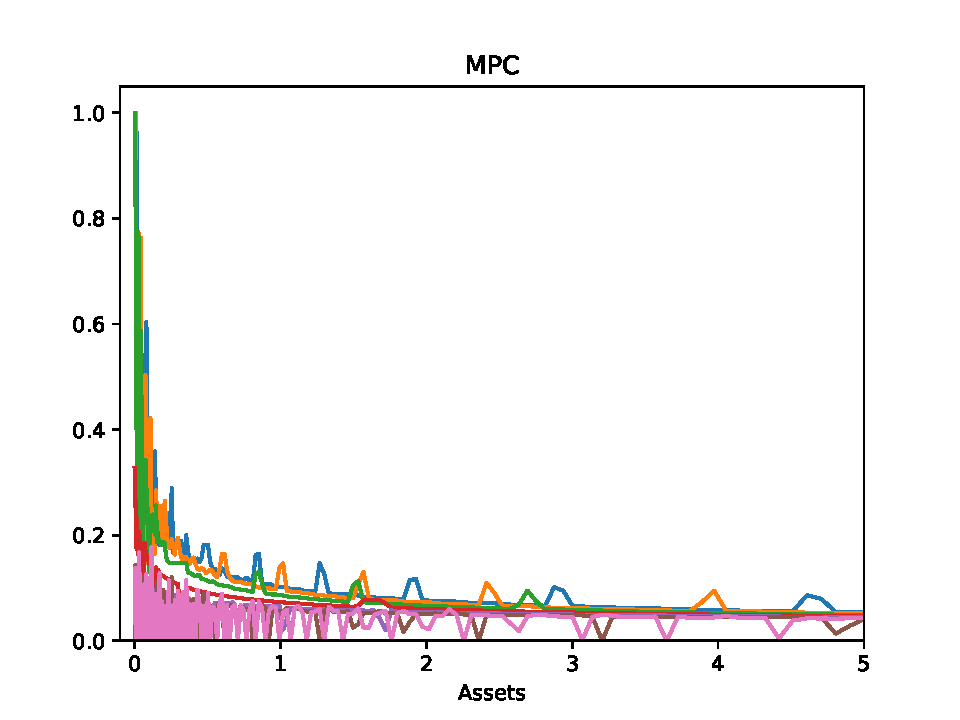
\includegraphics[width=0.48\textwidth]{figs/bs_MPC} & 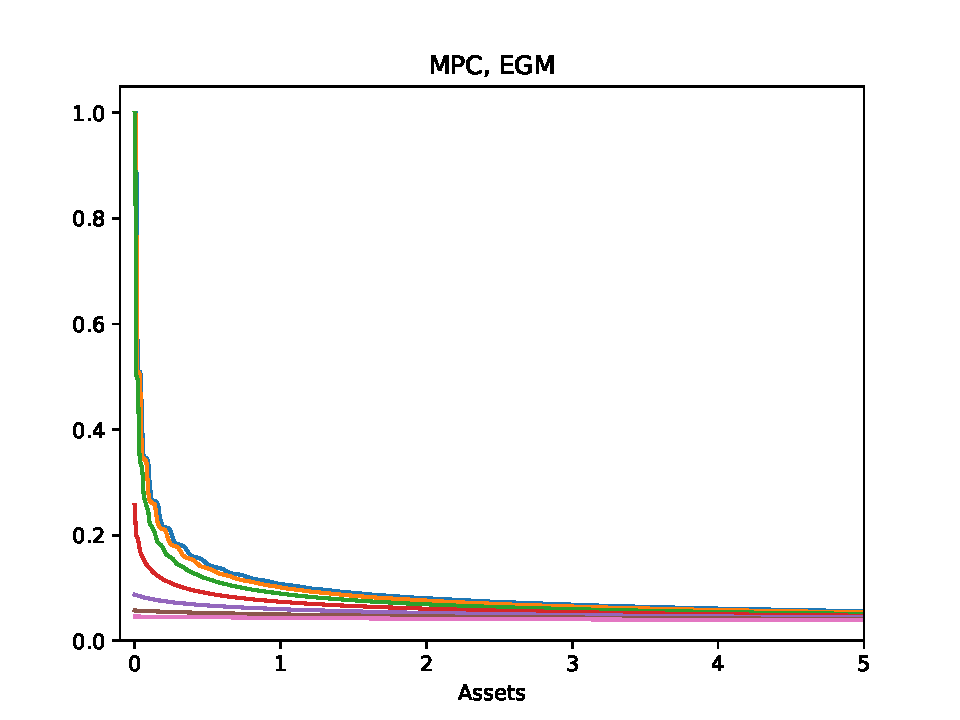
\includegraphics[width=0.48\textwidth]{figs/egm_MPC}\tabularnewline
\end{tabular}

\vspace{-1mm}
\begin{itemize}
\item <+->\textbf{Same model, same MPC, computed the same way }(first difference
of $c$ along the grid)
\item <+->\textbf{Left, VFI: }ragged. $\breve{v}$ is piecewise linear, so $a_{t}$
gets pinned at grid points
\item <+->\textbf{Right, EGM: }clean
\item <+->\textbf{On the deterministic problem: }EGM is exact at $\#_{a}=25$,
VFI needs hundreds of points for three digits
\end{itemize}
\end{frame}

\section{Simulation and aggregation}
\begin{frame}{From policy functions to aggregates}
\begin{itemize}
\item <+->\textbf{What we have: }$c^{\ast}(z_{t},a_{t-1})$ and $a^{\ast}(z_{t},a_{t-1})$,
what \emph{one} household does in every state
\item <+->\textbf{What the next lecture needs: }aggregates, e.g.\vspace{-1mm}
\[
A^{hh}_{t}=\sum_{i_{z}}\sum_{i_{a-}}\boldsymbol{D}_{t}(z^{i_{z}},a^{i_{a-}})\,a^{\ast}(z^{i_{z}},a^{i_{a-}})
\]
where $\boldsymbol{D}_{t}$ is the \emph{distribution} of households
over $\mathcal{G}_{z}\times\mathcal{G}_{a}$
\item <+->\textbf{So we need to simulate the distribution forward. }Two ways:
\begin{enumerate}
\item Monte Carlo: simulate $N$ households, average
\item Histogram (Young, 2010): iterate on $\boldsymbol{D}_{t}$ itself
\end{enumerate}
\item <+->\textbf{Notebook: }\texttt{05\_simulation.ipynb}
\end{itemize}
\end{frame}
%
\begin{frame}{Monte Carlo simulation}
\begin{itemize}
\item <+->\textbf{Initial distribution: }draw $z_{i,-1}$ and $a_{i,-1}$ for
$i\in\{0,1,\dots,N-1\}$
\item <+->\textbf{Simulation: }forwards in time from $t=0$, in each period
\begin{enumerate}
\item Draw $z_{it}$ given $z_{it-1}$ from the transition probabilities
\item Use linear interpolation to evaluate\vspace{-1mm}
\[
a_{it}=a^{\ast}(z_{it},a_{it-1})
\]
\end{enumerate}
\item <+->\textbf{Aggregation: }sample averages, $A^{hh}_{t}=\frac{1}{N}\sum_{i}a_{it}$
\begin{itemize}
\item Law of large numbers: correct as $N\rightarrow\infty$
\end{itemize}
\item <+->\textbf{Pro: }simple to implement, works for any model
\item <+->\textbf{Con: }computationally costly, and \emph{random}
\end{itemize}
\end{frame}
%
\begin{frame}{Monte Carlo noise}

\begin{tabular}{@{}c@{\hspace{2mm}}c@{}}
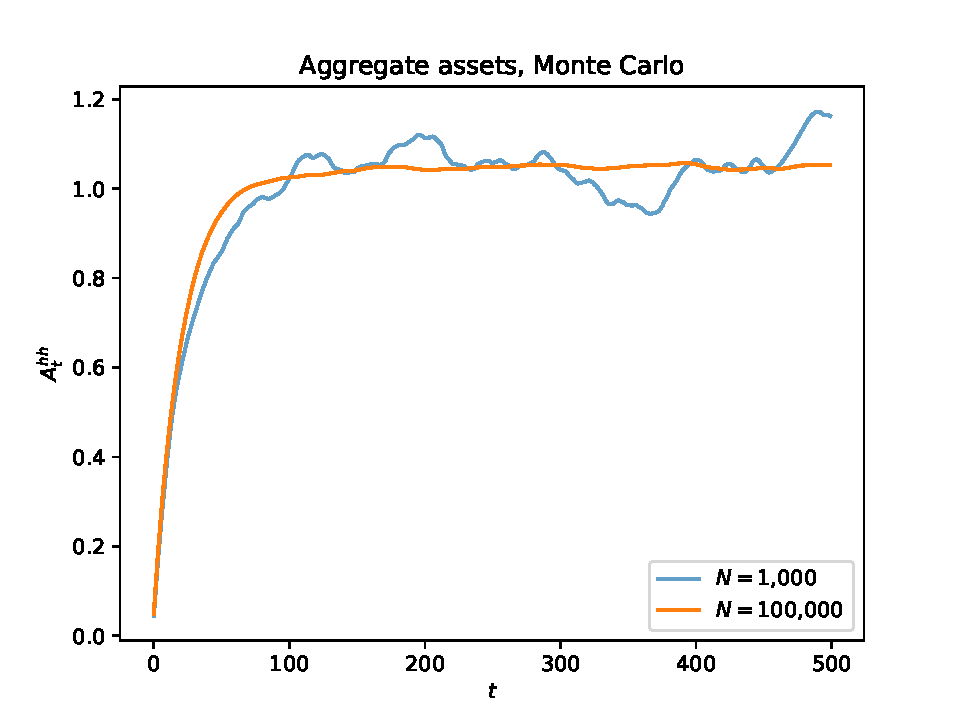
\includegraphics[width=0.48\textwidth]{figs/sim_mc_A} & 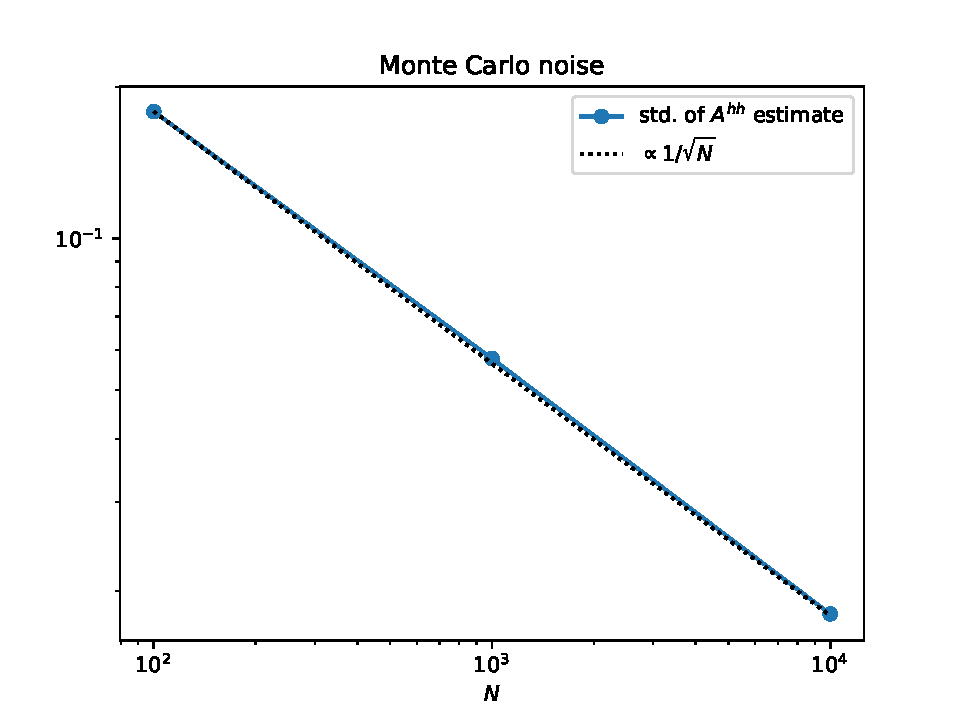
\includegraphics[width=0.48\textwidth]{figs/sim_mc_noise}\tabularnewline
\end{tabular}

\vspace{-1mm}
\begin{itemize}
\item <+->\textbf{Left: }$A^{hh}_{t}$ never settles, it keeps fluctuating around
its stationary level
\item <+->\textbf{Right: }the error falls like $1/\sqrt{N}$: quadrupling $N$
halves it
\item <+->\textbf{Why this hurts: }next lecture we root-find on asset market
clearing, $A^{hh}(r)-K(r)=0$. A stochastic $A^{hh}$ puts a floor
on the achievable tolerance
\end{itemize}
\end{frame}
%
\begin{frame}{The distribution as an object}
\begin{itemize}
\item <+->\textbf{Idea: }stop tracking households, track \emph{probability mass}
\item <+->\textbf{Histogram: }an array $\boldsymbol{D}$ on $\mathcal{G}_{z}\times\mathcal{G}_{a}$,
summing to $1$
\begin{itemize}
\item $\underline{\boldsymbol{D}}_{t}$: beginning-of-period, over $(z_{t-1},a_{t-1})$
\item $\boldsymbol{D}_{t}$: after the productivity draw, over $(z_{t},a_{t-1})$
\end{itemize}
\item <+->\textbf{The productivity transition is exact:}\vspace{-1mm}
\[
\boldsymbol{D}_{t}(z^{i_{z}},a^{i_{a-}})=\sum_{i_{z-}}\pi_{i_{z-},i_{z}}\underline{\boldsymbol{D}}_{t}(z^{i_{z-}},a^{i_{a-}})\iff\boldsymbol{D}_{t}=\Pi^{\prime}_{z}\underline{\boldsymbol{D}}_{t}
\]
\item <+->\textbf{The problem: }all mass at $(z^{i_{z}},a^{i_{a-}})$ saves $a^{\ast}(z^{i_{z}},a^{i_{a-}})$,
which falls \emph{between} grid points
\end{itemize}
\end{frame}
%
\begin{frame}{The savings lottery}
\begin{itemize}
\item <+->\textbf{Split the mass between the two neighbors. }Find $i$ such that
$a^{i}\leq a^{\ast}\leq a^{i+1}$ and set\vspace{-1mm}
\[
\omega=\frac{a^{i+1}-a^{\ast}}{a^{i+1}-a^{i}}\in[0,1]
\]
\item <+->\textbf{Assign }share $\omega$ to $a^{i}$ and $1-\omega$ to $a^{i+1}$
\begin{itemize}
\item The lottery has mean \emph{exactly} $a^{\ast}$: aggregate savings
are not distorted by the grid
\end{itemize}
\item <+->\textbf{One full period:}\vspace{-1mm}
\[
\underline{\boldsymbol{D}}_{t}\overset{\Pi^{\prime}_{z}}{\longrightarrow}\boldsymbol{D}_{t}\overset{\Lambda^{\prime}}{\longrightarrow}\underline{\boldsymbol{D}}_{t+1}
\]
where $\Lambda$ collects the lottery weights
\item <+->\textbf{Both maps are linear and deterministic: }simulation becomes
matrix algebra. No draws, no noise
\end{itemize}
\end{frame}
%
\begin{frame}{Monte Carlo vs histogram}

\begin{center}
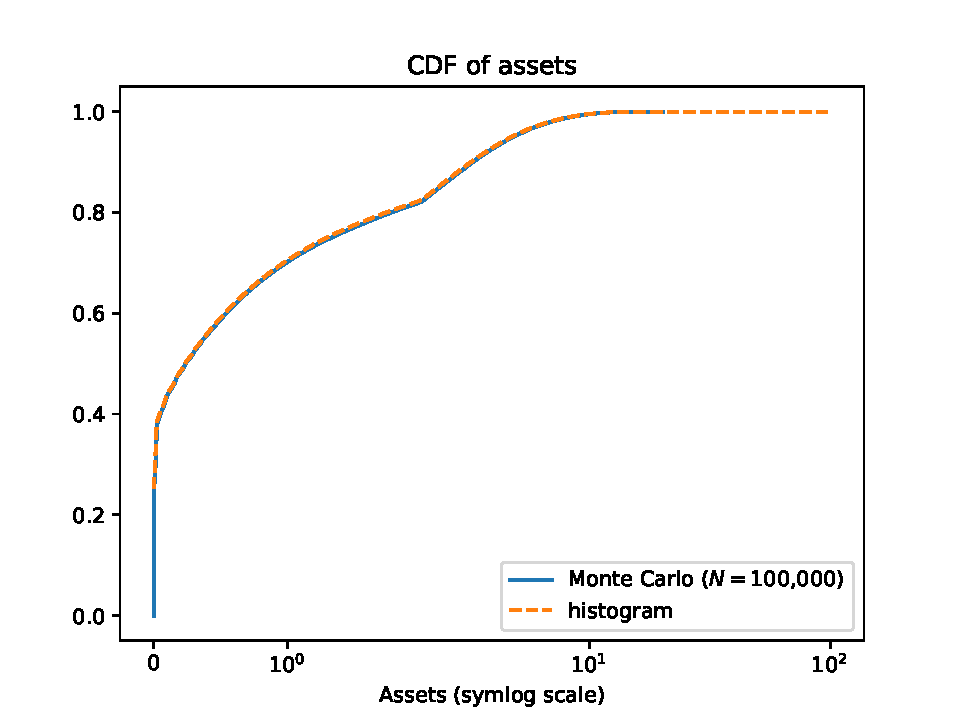
\includegraphics[width=0.72\textwidth]{figs/sim_mc_vs_hist}
\end{center}

\vspace{-2mm}
\textbf{Same distribution. }The histogram is the exact limit the Monte
Carlo approaches by brute force, at a fraction of the cost. Its only
cost: the distribution lives \emph{on the grid}.
\end{frame}
%
\begin{frame}{Aggregation}
\begin{itemize}
\item <+->\textbf{Aggregates are sums over the grid:}\vspace{-1mm}
\[
A^{hh}=\sum_{i_{z},i_{a-}}\boldsymbol{D}(z^{i_{z}},a^{i_{a-}})\,a^{\ast}(z^{i_{z}},a^{i_{a-}}),\qquad C^{hh}=\sum_{i_{z},i_{a-}}\boldsymbol{D}\,c^{\ast}
\]
\item <+->\textbf{Stationary distribution: }iterate the forward step until $\underline{\boldsymbol{D}}$ stops moving (526 iterations, $0.01$ secs)
\end{itemize}
\end{frame}

\section{Summary}

\begin{frame}{The household block in practice}
\begin{enumerate}
\item <+->\textbf{Backward step (EGM): }iterate\vspace{-1mm}
\[
\underline{v}_{a}\rightarrow c^{\ast}(z_{t},a_{t-1}),\,a^{\ast}(z_{t},a_{t-1})
\]
until the policy functions converge $\Rightarrow$ \lstinline{solve_hh_backwards}
\item <+->\textbf{Forward step (histogram): }build the lottery from $a^{\ast}$, iterate\vspace{-1mm}
\[
\underline{\boldsymbol{D}}_{t}\overset{\Pi^{\prime}_{z}}{\longrightarrow}\boldsymbol{D}_{t}\overset{\Lambda^{\prime}}{\longrightarrow}\underline{\boldsymbol{D}}_{t+1}
\]
until the distribution converges $\Rightarrow$ \lstinline{simulate_hh_forwards}
\item <+->\textbf{Aggregate: }$A^{hh}=\sum\boldsymbol{D}\,a^{\ast}$, $C^{hh}=\sum\boldsymbol{D}\,c^{\ast}$
\end{enumerate}
\vspace{2mm}
\textbf{This pair is the household block. }Next lecture
\lstinline{GEModelTools} runs it for us, and $r$ and $w$ become equilibrium objects.
\end{frame}
%
\begin{frame}{What you should remember}
\begin{enumerate}
\item <+->\textbf{The PIH gives an MPC of about }$2\%$\textbf{; the data say
}$40-50\%$
\item <+->\textbf{Uncertainty plus a borrowing constraint fixes it}
\item <+->\textbf{EGM solves the household problem fast and accurately}
\item <+->\textbf{The histogram method gives a precise distribution, }without simulation noise
\end{enumerate}
\vspace{3mm}
\textbf{Next: }\emph{Stationary equilibrium}

\vspace{3mm}
\textbf{You should:}
\begin{enumerate}
\item <+->Study the code from this lecture
\item <+->Glance at Aiyagari (1994), \\
>>Uninsured Idiosyncratic Risk and Aggregate Saving<<
\end{enumerate}
\end{frame}

\section{Misc}
\begin{frame}{1. Life-cycle (I)}
\begin{itemize}
\item <+->\textbf{Basically:}
\begin{enumerate}
\item Born, working, retired, die
\item Age-varying parameters (esp. income)
\end{enumerate}
\item <+->\textbf{Add-ons:}
\begin{enumerate}
\item Labor supply, human capital, occupation
\item Portfolio choice and entrepreneurship
\item Family formation
\item Health, mortality
\item []etc.
\end{enumerate}
\item <+->\textbf{Good starting example:} >>Life‐Cycle Consumption and Children:
Evidence from a Structural Estimation<<, Jørgensen (2017)
\end{itemize}
\end{frame}
%
\begin{frame}{1. Life-cycle (II)}

\vspace{-2mm}
\begin{columns}[T] % align columns
\begin{column}{.55\textwidth}

\textbf{Paper:} Gourinchas and Parker (2002)

\emph{Life-cycle consumption-saving model with retirement}
\begin{itemize}
\item <+->Young households: \\
Save for precautionary reasons (buffer)
\item <+->Older households:\\
Save for retirement (life-cycle)
\end{itemize}
\end{column}

\begin{column}{.55\textwidth}

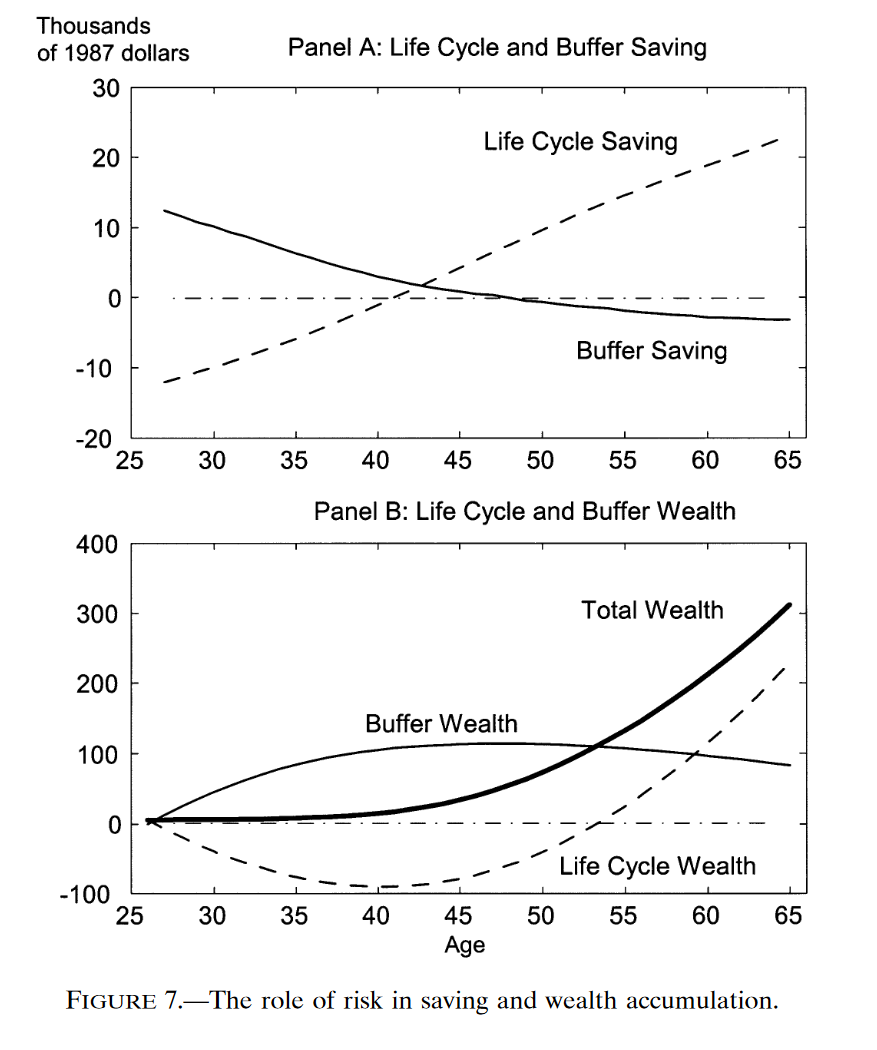
\includegraphics[width=1\textwidth]{figs/GourchasParker}

\end{column}

\end{columns}
\end{frame}
%
\begin{frame}{1. Life-cycle (III)}
\begin{itemize}
\item <+->\textbf{Natural experiment:} Wealth depletion after sudden inheritance
\item <+->\textbf{Results:}
\begin{enumerate}
\item Life-cycle profile of wealth fitted for many levels of risk-aversion\\
(by varying the discount factor)
\item Fast wealth depletion requires high risk-aversion\\
(or high perceived risk)
\end{enumerate}
\end{itemize}
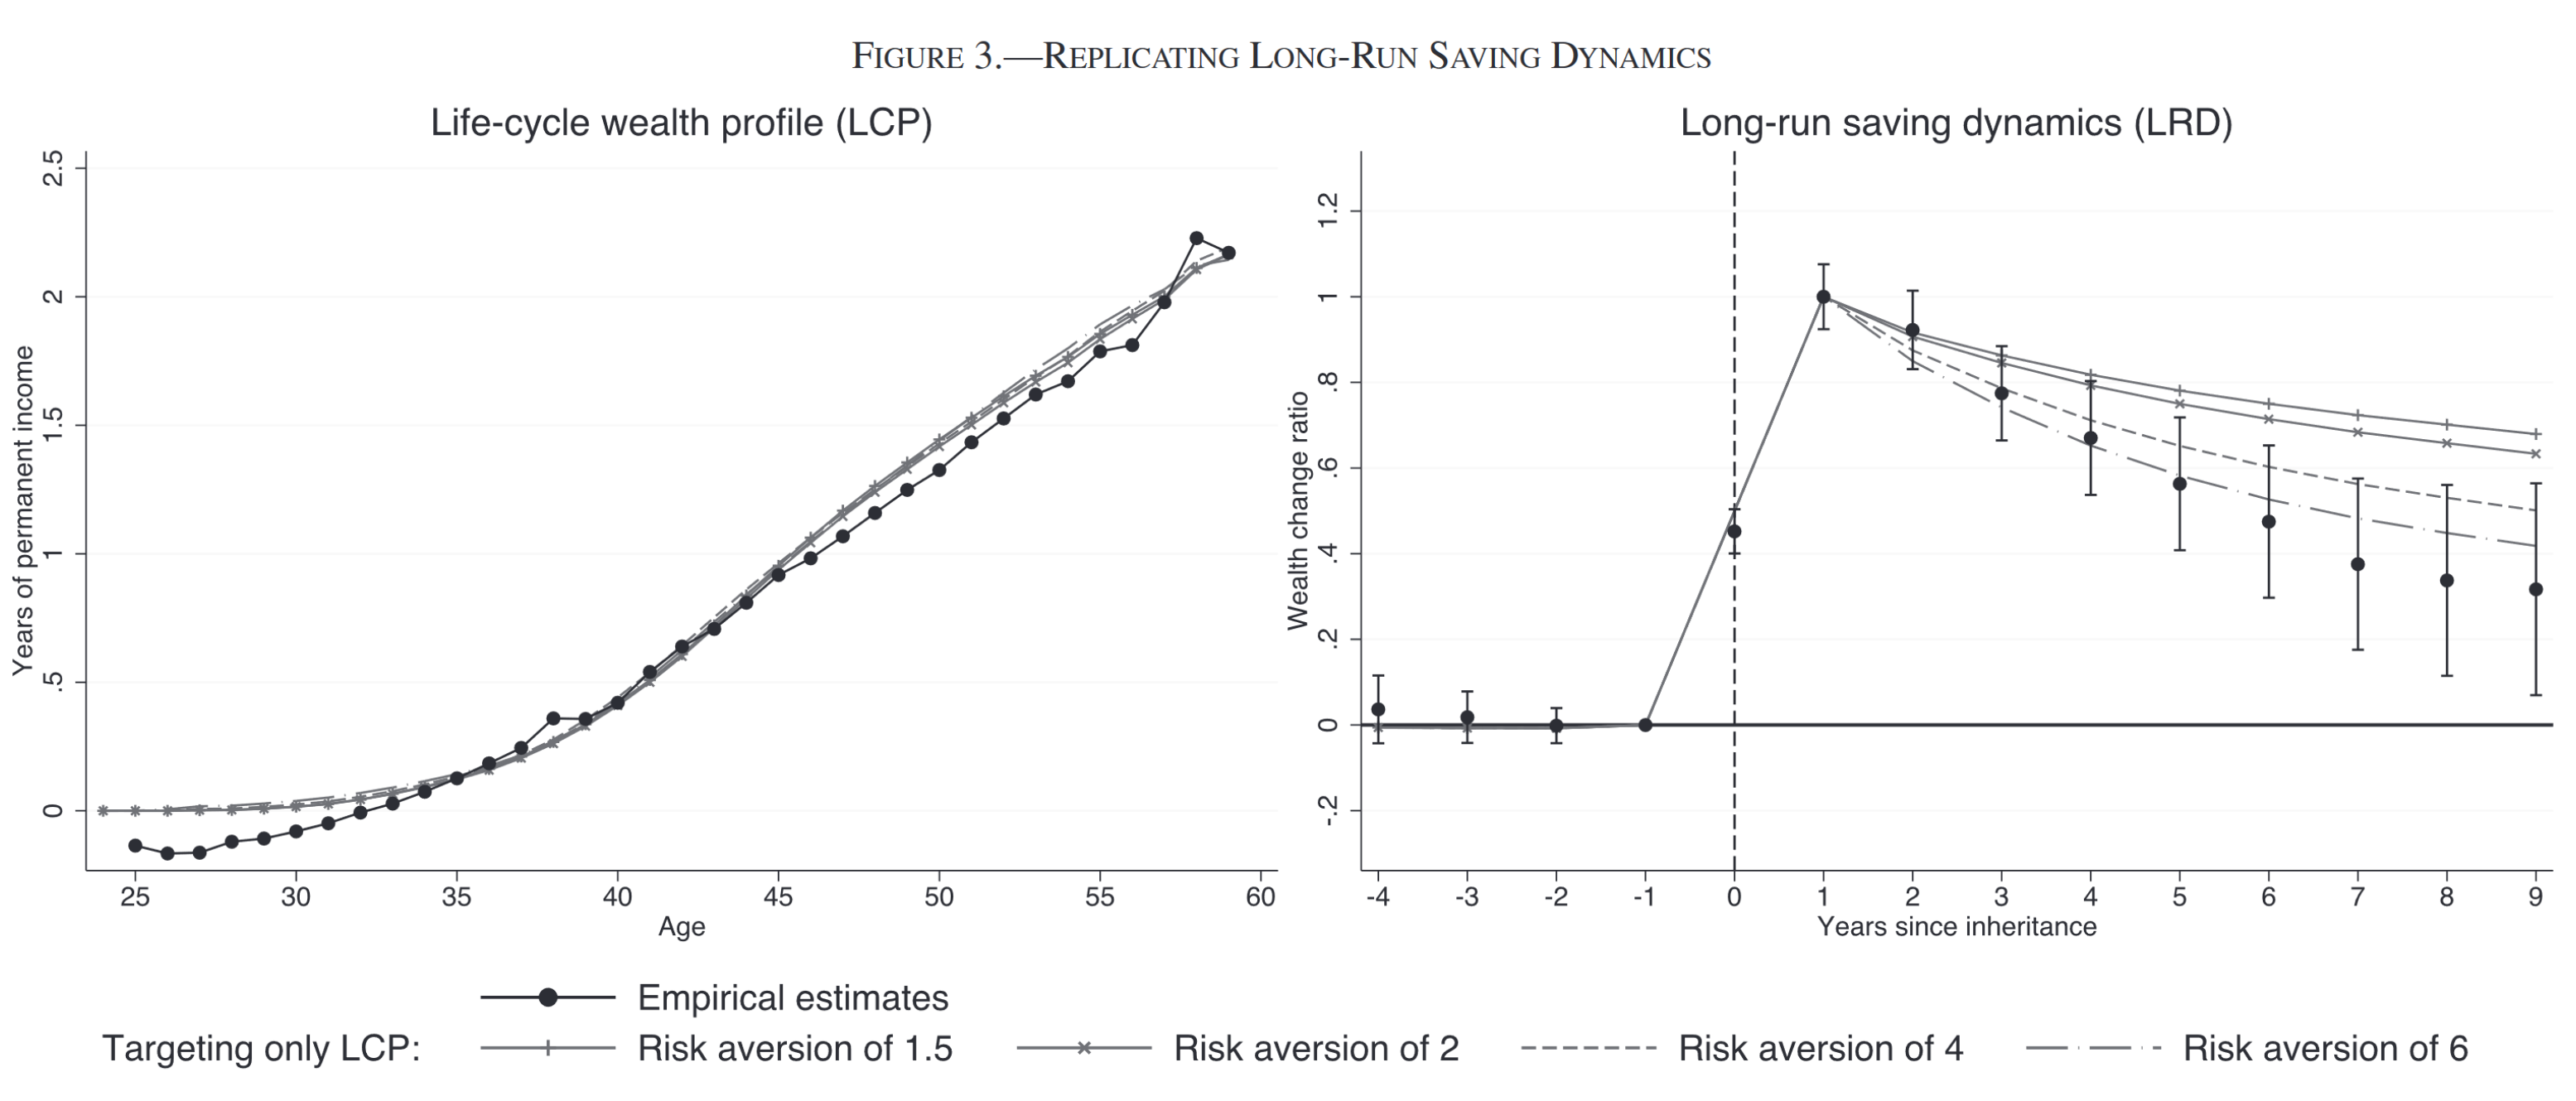
\includegraphics[width=0.95\textwidth]{figs/Druedahl_Martinello}\\
Source: Druedahl and Martinello (2022)
\end{frame}
%
\begin{frame}{2. More realistic income risk (I)}

Annual earnings-changes are far from log-normal:

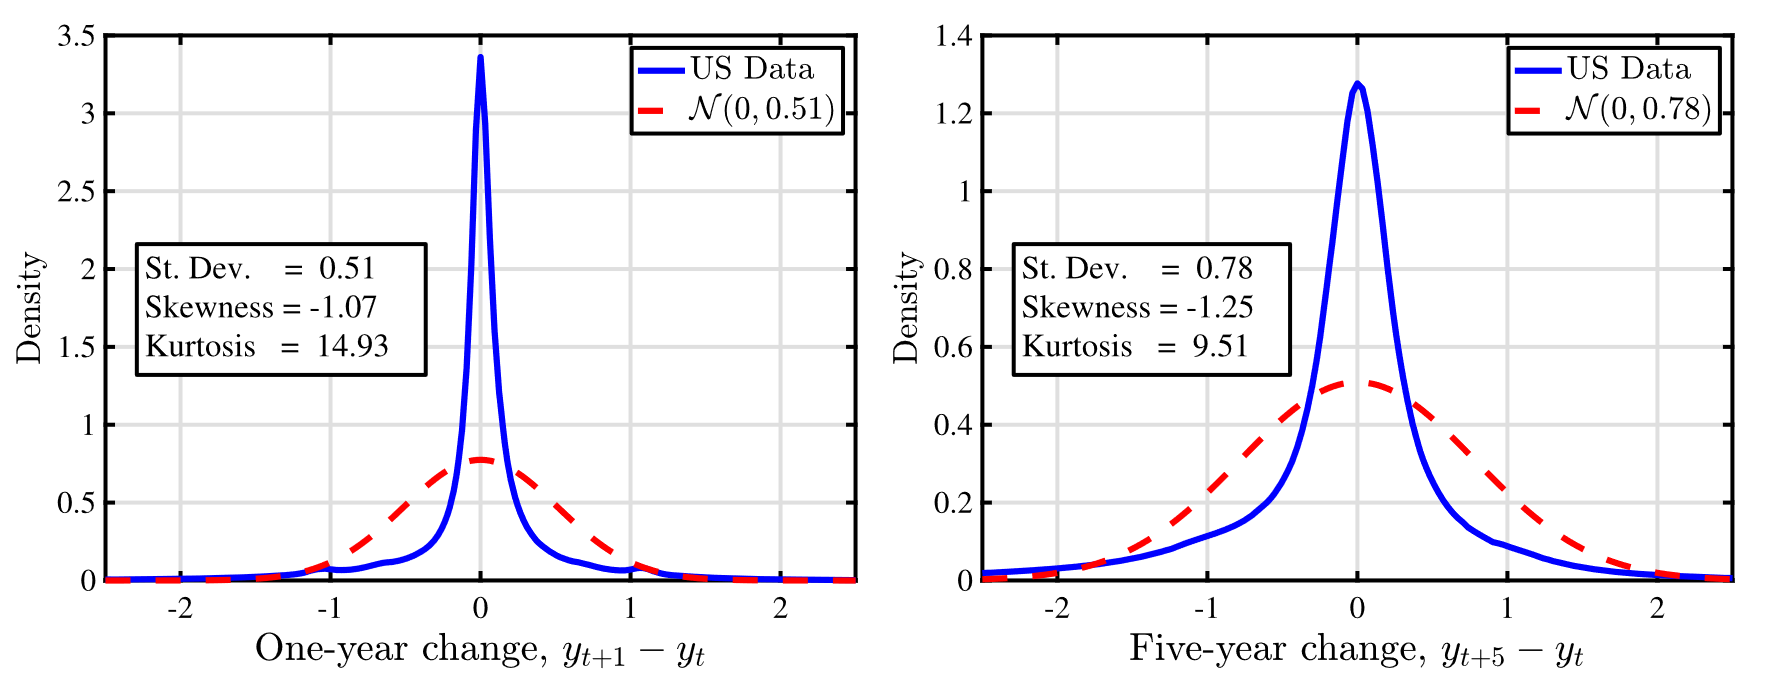
\includegraphics[width=1\textwidth]{figs/Guvenen}

Source: Guvenen et al. (2021)
\end{frame}
%
\begin{frame}{2. More realistic income risk (II)}

Many with zero-growth month-month:

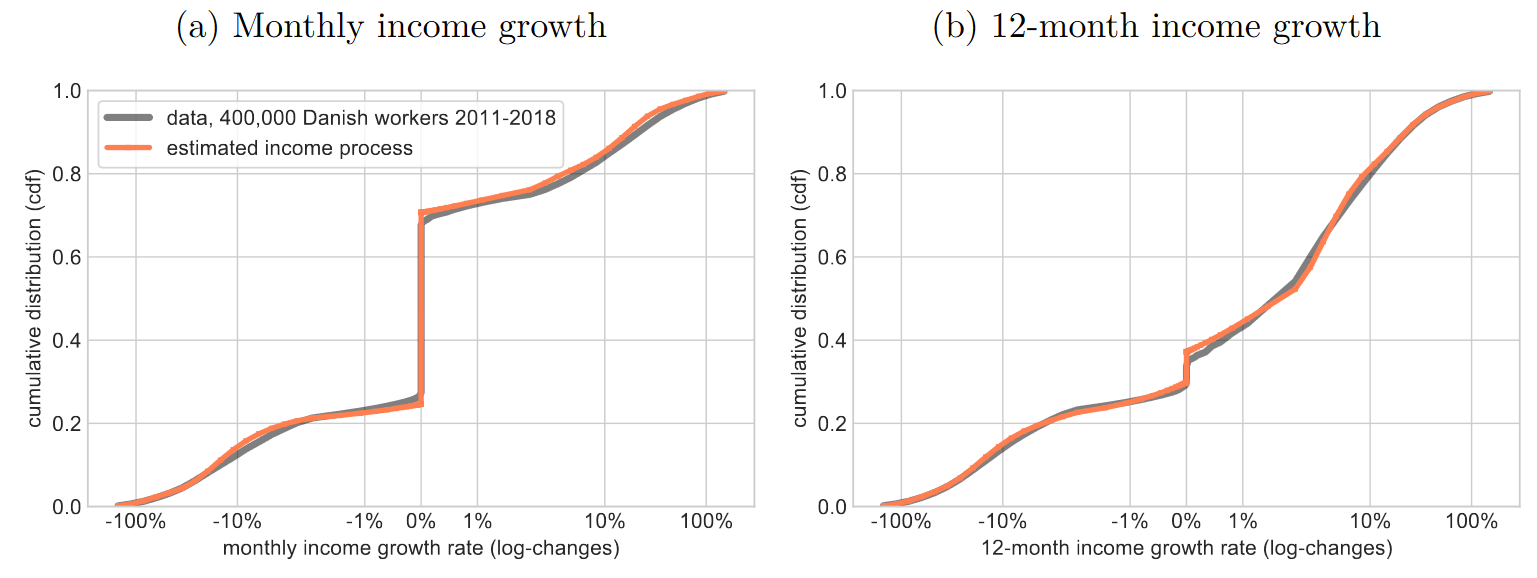
\includegraphics[width=1\textwidth]{figs/HighFreqIncDyn}

Source: Druedahl et al. (2021)
\end{frame}
%
\begin{frame}{3. Epstein-Zin}

\vspace{-6mm}
\begin{align*}
v_{t}\left(z_{t},m_{t}\right) & = & \max_{c_{t}}\left[\left(1-\beta\right)\cdot c^{1-\sigma}_{t}+\beta\cdot w^{1-\sigma}_{t+1}\right]^{\frac{1}{1-\sigma}}\\
 & \text{s.t.} & \,\,\,w_{t+1}\equiv\mathbb{E}_{t}\left[v_{t+1}\left(z_{t+1},m_{t+1}\right)^{1-\rho}\right]^{\frac{1}{1-\rho}}\\
 &  & \,\,\,m_{t+1}=(1+r)(m_{t}-c_{t})+y_{t+1}
\end{align*}

\begin{itemize}
\item <+->\vspace{-4mm}\textbf{Preferences:}
\begin{enumerate}
\item Patience: $\beta$
\item Intertemporal substitution: $\sigma$
\item Risk-aversion: $\rho$
\end{enumerate}
\item <+->\textbf{Euler-equation:} $c^{-\sigma}_{t}=\beta R\cdot\mathbb{E}_{t}\left[c^{-\sigma}_{t+1}\cdot\left(\frac{w_{t+1}}{v_{t+1}}\right)^{\rho-\sigma}\right]$\vspace{2mm}
\begin{enumerate}
\item FOC: $0=v^{\sigma}_{t}\cdot\left[\left(1-\beta\right)\cdot c^{-\sigma}_{t}-\beta R\cdot w^{\rho-\sigma}_{t+1}\cdot\mathbb{E}_{t}\left[v^{-\rho}_{t+1}\cdot\frac{\partial v_{t+1}}{\partial m_{t+1}}\right]\right]$\vspace{1mm}
\item Envelope condition: $\frac{\partial v_{t}\left(z_{t},m_{t}\right)}{\partial m_{t}}=v^{\sigma}_{t}\cdot\left(1-\beta\right)\cdot c^{-\sigma}_{t}$
\end{enumerate}
\end{itemize}
\end{frame}
%
\begin{frame}{4. Deep learning}
\begin{itemize}
\item <+->\textbf{Curse of dimensionality: }
\begin{enumerate}
\item Many states
\item Many choices
\item Many shocks
\end{enumerate}
\item <+->\textbf{Deep (reinforcement) learning:}
\begin{enumerate}
\item Approximate value and policy functions with \emph{neural networks}
\item Approximate on simulation sample rather than on grid
\item Automatic differentiation (backpropagation) and GPUs for speed
\end{enumerate}
\item <+->\textbf{Examples:} Maliar and Maliar (2021) and Azinovic and Scheidegger
(2022)
\item <+->\textbf{Working paper:} Druedahl and Røpke (2025)

Python package: {\color{DarkRed}\href{https://github.com/NumEconCopenhagen/EconDLSolvers}{EconDLSolvers}}
\end{itemize}
\end{frame}
%

\end{document}
